\documentclass[a4paper,10pt]{article}

\usepackage[pages=all, color=black, position={current page.south}, placement=bottom, scale=1, opacity=1, vshift=5mm]{background}
\SetBgContents{
} 
\usepackage[margin=0.92in]{geometry} 




\title{Moderate-length lifted quantum Tanner codes}
\author{Virgile Guemard$^{1, 2}$ \and Gilles Zemor$^{3,4}$}

\date{
	$^1$Aix Marseille Université, I2M, UMR 7373, 13453 Marseille, France\\%
        $^2$Inria Paris, France \\
        $^3$Institut de Mathématiques de Bordeaux, UMR 5251\\
        $^4$Institut universitaire de France\\[2ex]%
	\today
}
 \newcommand{\CG}{\mathcal{G}\xspace}
\newcommand{\CV}{\mathcal{V}\xspace}
\newcommand{\CE}{\mathcal{E}\xspace}
\newcommand{\CA}{\mathcal{A}\xspace}
\newcommand{\CF}{\mathcal{F}\xspace}
\newcommand{\CR}{\mathcal{R}\xspace}
\newcommand{\CB}{\mathcal{B}\xspace}
\newcommand{\CX}{\mathcal{X}\xspace}
\newcommand{\CK}{\mathcal{K}\xspace}
\newcommand{\CM}{\mathcal{M}\xspace}
\newcommand{\CC}{\mathcal{C}\xspace}
\newcommand{\CL}{\mathcal{L}\xspace}
\newcommand{\CI}{\mathcal{I}\xspace}
\newcommand{\CQ}{\mathcal{Q}\xspace}
\newcommand{\CO}{\mathcal{O}\xspace}
\newcommand{\CP}{\mathcal{P}\xspace}
\newcommand{\CS}{\mathcal{S}\xspace}
\newcommand{\CT}{\mathcal{T}\xspace}
\newcommand{\CJ}{\mathcal{J}\xspace}
\usepackage[para]{footmisc}
\usepackage{subfig}
% \usepackage{subcaption}
% \usepackage{array}
% \usepackage{colortbl}



 
\begin{document}
	\maketitle

\begin{abstract}
We introduce new families of quantum Tanner codes, a class of quantum codes which first appeared in the work of Leverrier and Z\'emor \cite{Leverrier2022}. These codes are built from two classical Tanner codes, for which the underlying graphs are extracted from coverings of 2D geometrical complexes, and the local linear codes are tensor-product of cyclic or double-circulant linear codes. We present several explicit families, and identify instances of moderate length quantum codes which are degenerate, have low check weight, and for which the distance surpasses the square root of the code length. Among them, we report the existence of a $[[96,2,12]]$ code, for which half of the checks are of weight 8 and the other half of weight 4.
\end{abstract}

\section{Introduction}

Quantum error correcting codes are believed to be unavoidable constituents of quantum computing architectures. Among them, quantum low-density parity-check (LDPC) codes are the leading candidates for physical implementations, because their low connectivity translates into a limitation of the error propagation between the hardware constituents. Significant progress has been made recently in the construction of good quantum LDPC codes \cite{Panteleev2021,Leverrier2022,LinHsie2022}, i.e. codes families with constant rate and relative distance in the asymptotic limit. These families can constitute a valuable source of inspiration to devise new types of codes of moderate length, following the effort in the design of near term implementable codes \cite{Panteleev2020,Pryadko2022,Bravyi2024}. \par

In 2022, Leverrier and Z\'emor \cite{Leverrier2022} generalized the Sipser-Spielman version \cite{Sipser1996} of  classical Tanner codes \cite{Tanner1981ARA} to devise a new family of asymptotically good Calderbank, Shor, Steane (CSS) codes that they call quantum Tanner codes. The methodology of \cite{Tanner1981ARA} relies on two components: a family of geometrical complexes and a set of short linear codes. It is instantiated by considering 2D square-complexes called left-right Cayley complexes, first used in the coding context in \cite{Dinur2021}. Given one of these complexes, its face-vertex incidence structure can generate two graphs, each of which is used to define a classical Tanner code. The local structure of the complex suggests classical tensor-product codes as a natural choice for the local linear codes of these Tanner codes. Although this CSS construction is state of the art in the asymptotic regime, short-length examples based on the same ideas have not yet been developed.\par

In this article, we introduce new types of quantum Tanner code families, taking inspiration of the Leverrier-Z\'emor construction. The main novelty of our approach is that we start by defining a quantum Tanner code on a square-complex, which is not necessarily a left-right Cayley complex, or a constant-degree graph as in \cite{Mostad2024}. We then use it to build larger codes based on the idea of code lifting.\par

In classical coding theory, lifting \cite{Thorpe2003} is a natural and practical method to generate new codes from old ones. Lifting a code corresponds to taking a covering of its Tanner graph representation. This strategy has proven to be very successful in producing LDPC codes of various blocklengths, and is now also applied to generate LDPC codes used in the 5G New Radio \cite{Richardson2018}. Moreover, the optimal Sipser-Spielman expander code family \cite{Sipser1996} designed in \cite{Panteleev2021} can be generated by a constrained version of the lift, called \textit{lift of Tanner code} in this article.\par

It is hence natural to consider lifting constructions for quantum LDPC codes. For CSS codes, a notion of lift was defined in \cite{guemard2024liftsquantumcsscodes}, based on the idea of covering spaces over a 2D complex associated with a given CSS code. \par
In the present article, we extend this notion to generate families of large Tanner codes from small ones. Our approach is a generalization of the classical lift of Tanner codes, which was used in \cite{Panteleev2021} to generate the optimal classical codes involved in their lifted product. Here, instead of using only a graph and a local code, we need a 2-dimensional square-complex over which two classical Tanner codes can be defined, forming an input CSS code. Then a covering of the square-complex allows us to simultaneously define lifts for these two classical Tanner codes. The maximum weight of the rows and columns of the lifted check matrices is equal to that of the input code, making it ideal for LDPC constructions. The weakness of our method is that lifting a CSS code does not always yield a valid CSS code. This is because the symmetries of the local codes must be adapted to the structure of the underlying 2D complex.\par

We illustrate the lifting of quantum Tanner code on explicit examples. In our previous work \cite{guemard2024liftsquantumcsscodes}, new code constructions were introduced using certain 2D geometrical complexes, namely square subdivisions of presentation complexes of finitely presented groups; the CSS codes were built by interpreting vertices, in the subdivision of these complexes, as parity checks and qubits. Here, following \cite{Leverrier2022}, we modify our point of view and interpret the faces as qubits. The novelty of our method is to first construct a short length quantum Tanner code on these subdivided complexes by fixing a specific configuration of the local codes. We then obtain our lifted Tanner code by generating coverings of these square-complexes, and by lifting the local code configuration on the covering spaces. In certain cases, the effect of the local code is to suppress the local codewords, causing the support of minimal codewords to be spread out in the complex. In this manner, we are able to obtain instances of  LDPC codes for which the square of the distance is greater than the blocklength. Another consequence is that a lifted code inherits the symmetry group of its associated covering space. \par

It has proven challenging to determine analytically the parameters of our lifted Tanner codes. We hence choose to follow a numerical approach. For some chosen input quantum Tanner codes, we generate all possible lifts of index 1 to 30, producing codes with length less than 800 qubits. An upper bound for the distance is calculated with GAP and the package QDistRnd \cite{Pryadko2022}. We only report the codes with the best parameters and leave a more rigorous analysis for future work.\par


The article is organized as follows. In Section \ref{section Preliminaries}, we set the notation for graphs, square-complexes and covering maps. We also review classical Tanner codes and our preferred method for lifting them. \par

In Section \ref{section: quantum Tanner codes and their lifts} we present a method to lift a quantum Tanner code. The idea is a generalization of the lift of a classical Tanner code, in which the central object is a covering of a square-complex rather than a graph.\par

Lastly, Section \ref{section:New constructions of quantum Tanner codes} contains our main contribution.  There, we introduce two new constructions of quantum Tanner codes. We study the parameters of lifted codes numerically and report specific instances with the highest distance.

\section{Preliminaries}\label{section Preliminaries}

\subsection{Graphs and square-complexes}\label{Graphs, square-complexes and covering maps}

In this article, crucial components of the linear and quantum code constructions are graphs and square-complexes. We therefore set some notation and state elementary facts on these objects, which will be used throughout this article.\par

We denote by $\mathcal G:=(V,E)$ an undirected graph with set of vertices $V$ and edges $E$. An \textit{edge} between two vertices $u$ and $v$ is an unordered pair $\{u,v\}=\{v,u\}$. In this work, graphs have no loops unless otherwise stated, but they can have multi-edges. A \textit{directed edge} is an edge for which the order matters, written $e=[u,v]$ for an edge with source $u$ and target $v$. The inverse of an edge is defined as $[u,v]^{-1}:=[v,u]$. A path in the graph is a sequence of directed edges $\alpha=[u,v].[v,w]\dots $. The edge-neighborhood of a vertex $v$,  denoted $E(v)$, is the set of edges connected to $v$, and its cardinality is the degree of $v$.\par

A square-complex is defined as a graph with a set of preferred subgraphs which are \textit{4-cycles}, namely cycle-graphs with 4 edges. We denote it $\mathcal S:=(V,E,F)$, where $(V,E)$ is the underlying graph, also called its 1-skeleton, and $F$ is a set of 2D faces. We say that $\mathcal S$ is a \textit{bipartite square-complex} if $(V,E)$ is a bipartite graph. A face $f\in F$ can be described by its corresponding cycle graph, or by a circuit such as $\alpha_f=[v_1,v_2].[v_2,v_3].[v_3,v_4].[v_4,v_1]$. The face-neighborhood of a vertex $v$ is the set of faces to which it is incident and is denoted $F(v)$. Moreover, we say that two faces are adjacent in $\mathcal S$ if they share a common edge.\par

For considerations related to covering spaces in Section \ref{section covering maps}, it will be important to introduce the following notions. Define a \textit{circuit }starting at vertex $v_1$ as a succession of directed edges such as $e_1.e_2\dots e_n=[v_1,v_2].[v_2,v_3].\dots.[v_n,v_1]$. An elementary reduction of a circuit consists of either removing two consecutive terms $e_i$ and $e_j$ if $e_i=e_j^{-1}$, or removing four consecutive terms if the corresponding edges form a face $f\in F$. The equivalence relation generated by elementary reductions is called homotopy: it is compatible with concatenation of circuits, and the \textit{fundamental group} $\pi_1(S,v) $ is the set of homotopy classes of circuits starting at $v$, with concatenation as group operation. It can be shown that the groups $\pi_1(S,v)$ and $\pi_1(S,v')$ are isomorphic for any two choices of vertices $v$ and $v'$ if $(V,E)$ is a connected graph, and therefore we often omit this choice and write it $\pi_1(\mathcal S)$. If $\mathcal S$ has an empty set of faces, i.e. $\mathcal S$ is the connected graph $\mathcal G=(V,E)$, the fundamental group is a free group of rank\footnote{This is the smallest cardinality of a generating set of the group.} $|E|-|V|+1$. For a general square complex $\mathcal S=(V,E,F)$, this is the group $\pi_1(\mathcal G)/N$, where $N$ is the normal closure of the subgroup generated by the elements of $\pi_1(\mathcal G)$ corresponding to the 4-cycles of $F$.\par

The reader can also see $\mathcal S$ as a 2D cell complex \cite{HatcherTopo}, all of whose faces have a boundary which is a 4-cycle, endowed with the topology of a CW complex. In this setting, our notion of fundamental group is equivalent to the general one defined in algebraic topology. 

\subsection{Covering maps}\label{section covering maps}

We now review some results about covering maps from \cite{GROSS1977273, HatcherTopo, Lyndon2001}. While some of them apply to topological spaces in general, we will only consider them in the context of graphs and square-complexes of finite degrees with a single connected component.\par

We first summarize a graph covering construction which can generate all possible finite graph coverings, as shown in \cite{GROSS1977273}. Let $r>0$ be an integer and $S_r$ be the symmetric group on the set $[r]:=\{0,\dots,r-1\}$.  Given a graph $\mathcal G=(V,E)$, we first assign a permutation $\pi_e\in S_r$ to each oriented edge $e$ of $\mathcal G$, with the constraint that $\pi_{e^{-1}}=\pi_{e}^{-1}$. We construct a graph $\tilde{\mathcal G}$ with set of vertices in bijection with $V\times [r]$ and set of edges in bijection with $E\times [r]$, where an element $c$ of $\tilde{\mathcal G}$, vertex or edge, is written $(c,i)$ for $i\in [r]$. An edge $(e,i)$ in the graph $\tilde{\mathcal G}$, where $e=[u,v]$, connects $(u,i)$ and $(v,\pi_e (i ))$. It is then possible to define a \textit{covering map} $p:\tilde{\mathcal G}\rightarrow  \mathcal G$ acting on an element $(c,i)$, vertex or edge, by $p((c,i))=c$. The graph $\tilde{\mathcal G}$ is called an \textit{index-$r$ covering} of $\mathcal G$. A vertex $(v,i)$ and its projection $v$ have the same degree. Moreover, an edge $\tilde e=[\tilde u,\tilde v]$ projects onto an edge $e=[p(\tilde u),p(\tilde v)]$ .

Given a square complex $\mathcal S=(V,E,F)$, an index-$r$ covering $\tilde{\mathcal S}$ is a graph covering $p:\tilde{\mathcal G}\rightarrow  \mathcal G$ which does not break the faces, i.e if $\alpha$ is a 4-cycle in $\mathcal G$ describing a face of $F$, then $p^{-1}(\alpha)$ is a set of $r$ disjoint 4-cycles. The set of faces in the covering is in bijection with $F\times [r]$,  and given a face $f\in F$ described by the path $e_1.e_2.e_3.e_4=[v_1,v_2].[v_2,v_3].[v_3,v_4].[v_4,v_1]$, then for all $i\in [r]$, the face labeled $(f,i)$ in $\tilde{\mathcal S}$ can be described by the following 4-cycle,

\begin{center}
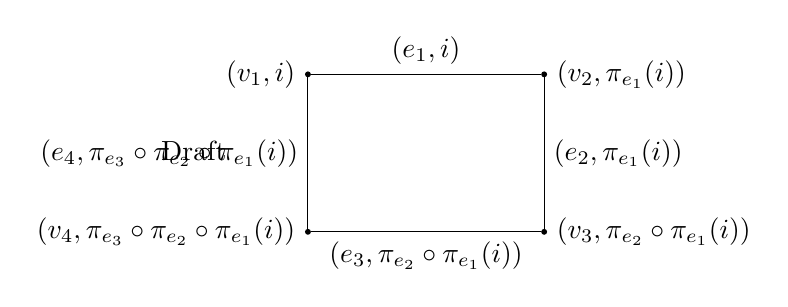
\begin{tikzpicture}
    % Nodes
    \node[draw, circle, fill=black, inner sep=0.6pt, label=left:{$(v_1,i)$}] (v1) at (0,2) {};
    \node[draw, circle, fill=black, inner sep=0.6pt, label=right:{$(v_2,\pi_{e_1}(i))$}] (v2) at (3,2) {};
    \node[draw, circle, fill=black, inner sep=0.6pt, label=right:{$(v_3,\pi_{e_2}\circ \pi_{e_1}(i))$}] (v3) at (3,0) {};
    \node[draw, circle, fill=black, inner sep=0.6pt, label=left:{$(v_4,\pi_{e_3}\circ\pi_{e_2}\circ \pi_{e_1}(i))$}] (v4) at (0,0) {};
    
    % Edges
    \draw (v1) -- node[above] {$(e_1,i)$} (v2);
    \draw (v3) -- node[right] {$(e_2,\pi_{e_1}(i))$} (v2);
    \draw (v3) -- node[below] {$(e_3,\pi_{e_2}\circ \pi_{e_1}(i))$} (v4);
    \draw (v4) -- node[left] {$(e_4,\pi_{e_3}\circ\pi_{e_2}\circ \pi_{e_1}(i))$} (v1);
\end{tikzpicture}
\end{center}
We can then define an index-$r$ covering map $p:\tilde{\mathcal S}\to \mathcal S$ acting on an element $(c,i)$ (vertex, edge or face) by $p((c,i))=c$, and therefore $p$ maps faces to faces. The inverse image of any vertex, edge or face is a set of $r$ vertices, edges or faces.\par

We now consider a square-complex $\mathcal S$, possibly with an empty set of faces, i.e. a graph. Given a covering $p:\tilde{\mathcal S}\to \mathcal S$, a \textit{deck transformation}\footnote{This name suggests an analogy to the mixing of a deck of cards, which are called sheets in the context of covering spaces.} is an automorphism $\psi:\tilde{\mathcal S}\rightarrow \tilde{\mathcal S}$ such that $p\circ \psi=p$. The set of deck transformations, endowed with the operation of composition of maps, forms a group denoted $\operatorname{deck}(p)$. It is called the \textit{group of deck transformations} and acts on the left on $\tilde{\mathcal S}$. A \textit{Galois covering} is a covering enjoying a left, free and transitive action of $\operatorname{deck}(p)$ on the fiber. For any Galois covering, $p:\tilde{\mathcal S}\rightarrow \mathcal S$, it can be shown that $\operatorname{deck}(p)\setminus \tilde{\mathcal S}\cong \mathcal S$.\par 
In the rest of this section, by a covering $p:\tilde{\mathcal S}\to \mathcal S$ we always mean a \textit{finite} \textit{connected} covering, i.e. one whose index is finite and for which $\tilde{\mathcal S}$ is also a connected complex. The following crucial results of this section apply in this context. \par

The theory of connected covering maps over a complex depends on the structure of its fundamental group in the following way. For every index $r$ subgroup $H $ of the fundamental group $\pi_1(\mathcal S)$ there exists an index $r$ covering $p:\mathcal S_H\to \mathcal S$, mapping the basepoint $\tilde v$ of $\mathcal S_H$ to $v$, and inducing an injective homomorphism $p_\#:\pi_1(\mathcal S_H,\tilde v)\to \pi_1(\mathcal S,v)$, such that $p_\#\pi_1(\mathcal S_H , \tilde v) = H$. A covering $p:\mathcal S_H\to \mathcal S$ is called \textit{Galois} or \textit{normal} when $H$ is a normal subgroup of $\pi_1(\mathcal S,v)$. All the coverings that we will study in Section \ref{section:New constructions of quantum Tanner codes} are of this form. It can be shown that, for such a covering map, we have the isomorphism $\operatorname{deck}(p)\cong\pi_1(\mathcal S,v)/H$. The most important result on coverings is the classification theorem known as the Galois correspondence, which we state in our restricted setting of finite index coverings of complexes with finitely many cells.\footnote{This theorem applies in a much broader context, but this is sufficient for our applications.}

\begin{theorem}[Galois correspondence]\label{Theorem Galois correspond}
For all $r\in \mathbb N$, there is a bijection between the set of basepoint-preserving isomorphism classes of index-$r$ connected covering spaces of a complex $\mathcal S$ and the set of index-$r$ subgroups of $\pi_1 (\mathcal S)$. Given such a covering $p:\tilde{\mathcal S}\to \mathcal S$, it is obtained by associating the subgroup $H=p_\#\pi_1 (\tilde{\mathcal S} )$ to the covering space $\tilde{\mathcal S}$. The index of the associated covering is equal to the index $[\pi_1(\mathcal S):H]$.
\end{theorem}
This theorem motivates our exhaustive searches of all possible Galois coverings in Section \ref{section:New constructions of quantum Tanner codes}. Using this correspondence, we also describe a procedure in Appendix \ref{appendix lift} specifically designed to generate the covering of a square complex associated to a given subgroup of its fundamental group.

\subsection{Tanner codes and their lifts}\label{section Tanner codes and their lifts}

In this section, we recall some definitions and set up notations related to linear codes. The central components of our quantum codes are classical Tanner codes. We review their construction and a method to lift them into larger codes.\par

We denote the parameters of a binary linear code $C\subseteq \mathbb{F}_2^n  $  as $[n,k,d]$, where $n$ its the length, $k$ its dimension and $d$ its distance, defined as $d=\min\limits_{c\in C\setminus \{0\} }|c|$. If $k=0$, our convention is to set $d=0$. In what follows, a linear code will be defined by the image of a linear map $g:\mathbb F_2^k\to \mathbb F_2^n$,  or the kernel of a linear map, $h:\mathbb F_2^n\to \mathbb F_2^m$, respectively represented in a preferred basis $B$ by a generator matrix $G:=\operatorname{Mat}_B (g)$, and a parity-check matrix $H:=\operatorname{Mat}_B (h)$. Given $x\in \mathbb F_2^n$, the vector $s=Hx$ is called the $syndrome$ of $x$.  The generator matrix of $C$ is the parity-check matrix of its dual $C^\perp=\{x\in \mathbb F_2^n\: :\: \forall c\in C, \langle x,c\rangle=0\}$. A code is called self-dual when $C^\perp=C.$\par

The central linear code construction of this article is the classical Tanner code of \cite{Tanner1981ARA}, which was made popular by Sipser and Spielman \cite{Sipser1996}.\par

Let $\mathcal G=(V,E)$ be a graph on $|E|=n$ edges. In the following $\mathbb{F}_2E:=\bigoplus_{e\in E}\mathbb{F}_2 e$ denote the space of formal linear combination of elements of the set $E$, playing the role of basis vectors. Given a vertex, $v$, the space $\mathbb F_2E(v)$, is the restriction of $\mathbb F_2E $ to the edge neighborhood of $v$. We define a set of binary \textit{local codes} $C_V:=(C_v )_{ v\in V}$ on the vertices of $\mathcal G$, where an element indexed by $v\in V$ is a code defined on the edge neighborhood of $v$, i.e. $C_v \subseteq \mathbb F_2E(v)$. For a vector $c\in \mathbb F_2 E$, we denote $c|_{E(v)} $ its restriction to the edge-neighborhood of $v$.
\begin{definition}[Classical Tanner code]\label{definition classical Tanner code}
Let $\mathcal G=(V,E)$ be a graph and $C_V=(C_v )_{ v\in V}$ be a set of binary local codes. We define the Tanner code associated to $\mathcal{G}$ and $C_V$ as
\[ T(\mathcal G,C_V)=\{ c\in \mathbb F_2E : c|_{E(v)}\in C_v\text{ for all }v\in V\}.\]
\end{definition}

A Tanner code can also be defined by the kernel of a parity-check matrix. Suppose that $C_v$ is the kernel of a map $h_v:\mathbb F_2E(v)\to \mathbb F_2^{m_v}$ and let $i_v: \mathbb F_2^{m_v}\to \bigoplus_{u\in V} \mathbb F_2^{m_u}$ be the canonical linear embedding map. The Tanner code $C=T(\mathcal G,C_V)$ is the kernel of the map $
h :\mathbb F_2 E\xrightarrow[]{} \bigoplus_{u\in V} \mathbb F_2^{m_u}$, defined on an edge between vertex $v$ and $w$ by
\begin{equation}\label{equation:tanner code map}
h (e)= i_v\circ h_v (e) + i_w\circ h_w (e),
\end{equation}
and extended by linearity over $\mathbb F_2 E$. All vector spaces being given with a prefered basis, $h_v$ can be represented by a matrix $H_v$ and $h$ by a matrix $H$. Denoting $w$, $w_v$, the maximum row-weight of $H$ and $H_v$, respectively, and $q,q_v$ their column-weight, we have \[ w=\max\limits_{v\in V }w_v, \quad \quad q\leq\max \limits_{ \{v,w\}\in E} q_v+q_w .\]
For linear codes, lifting is an operation of major interest that produces families of LDPC codes \cite{Thorpe2003}, possibly with linear dimension and distance. It is equivalent to a covering of the Tanner graph representation of the code. In this article, we focus on lifts of Tanner codes. In that case, out of the many possible lifts, there exists a preferred choice, that we call the \textit{lift of a Tanner code}, as we will not use other types of lifts. From now on, we consider a graph $\mathcal G$ that has no loops. Then, given a graph covering $p:\tilde{\mathcal G}\to \mathcal  G$, where $\tilde{\mathcal G}=(\tilde V,\tilde E)$, the linear extension $p_*$ of $p$ on the set of edges induces an isomorphism\footnote{In the context of coverings of cells complexes, $p_*$ acts on chains of  $\mathbb F_2\tilde E$ and $\mathbb F_2\tilde V$  in the cellular chain complex and is a chain map.} $\mathbb F_2\tilde E(\tilde v)\overset{p_*}{\cong} \mathbb F_2 E(v)$, for any $\tilde v\in p^{-1}(v)$, which by definition sends basis vectors to basis vectors, i.e. edges to edges. 
\begin{definition}[Lift of Tanner code]\label{definition Lift of classical Tanner code}
 Let $C=T(\mathcal G,C_V)$ and $p:\tilde{\mathcal G}\to \mathcal  G$ be a graph covering, with $\tilde{\mathcal G}=(\tilde V, \tilde E)$. For each vertex $\tilde {v}\in \tilde V$, we associate the code $C_{\tilde v}\subseteq \mathbb F_2E(\tilde v)$, such that $C_{\tilde v} \overset{p_*}{\cong} C_{p(v)}$. The lifted Tanner code associated to $p$ is the code $\tilde C=T(\tilde{\mathcal G},C_{\tilde V})$, where $C_{  \tilde V}= (C_{\tilde v})_{ \tilde v\in \tilde V}$. In other words,
\[ T(\tilde{\mathcal G},C_{\tilde V})=\{c\in \mathbb F_2 \tilde E \: :\: p_*(c|_{\tilde E(\tilde v)})\in C_{p(\tilde v)}, \text{for all }\tilde v\in \tilde V\} \]
\end{definition}
Using the notations of the previous definitions, suppose that for each $v\in V$, $C_v$ is the kernel of a map $h_v$ represented by a matrix $H_v$, as described below Equation \eqref{equation:tanner code map}. Given a complete parity-check matrix $H$ of the Tanner code $C$, we can construct a Tanner graph of $C$. In this context, by lifting we always mean that for any $\tilde v\in p^{-1}(v)$, we define the code $C_{\tilde v}$ as the kernel of a map $h_{\tilde v}$ represented by the matrix $H_{\tilde v}=H_v$. In this way, fixing a matrix representation $H$ induces a matrix representation $\tilde H$, the parity-check matrix of $\tilde C$, up to permutation of the rows. Denoting $\tilde w$, $\tilde q$ the maximum row and column-weight of $\tilde H$, we have that \begin{equation}\label{Equation: lift conserve degree}
    \tilde q=q, \quad \tilde w=w.
\end{equation}
This can also be deduced from the fact that the lift of a Tanner code is an example of lift of a classical code associated to a certain covering, not necessarily connected, over the Tanner graph associated to $H$.\par

An automorphism of a binary linear code $C$ is a permutation of the coordinates mapping $C$ to itself. The set of automorphisms of $C$ forms the group $\operatorname{Aut}(C)$.  In the case of a lifted Tanner code $\tilde C$, notice that the group of deck transformation of $p:\tilde{\mathcal G}\to \mathcal  G$ is a symmetry group of the Tanner graph associated to the parity-check matrix $\tilde H$ described above. Therefore, given an element $\psi \in \operatorname{deck}(p)$, a vector $x\in \mathbb F_2 \tilde E$ with syndrome $\tilde Hx=s$, there exists a permutation $\sigma$ of the syndrome coordinates such that $\tilde H\psi(x)=\sigma(s)$. As so, $ \operatorname{deck}(p)$ is a subgroup of $\operatorname{Aut}(\tilde C)$, with the property that each element in this subgroup is equivalent to a certain permutation of the checks.

\subsection{Local codes}\label{section:local codes}

Throughout this article, for an integer $\ell\geq 1$, we denote $[\ell]= \{ 0,\dots ,\ell-1\}$. The classical local codes that will constitute our Tanner codes are built as dual of tensor-product codes. The tensor-product of linear codes $C\subseteq \mathbb F_2^{\ell_C}$ and $D\subseteq \mathbb F_2^{\ell_D}$, is the linear code denoted $ \Pi=C\otimes D\subseteq \mathbb F_2^{\ell_C}\otimes \mathbb F_2^{ \ell_D}$. The canonical bases of $ \mathbb F_2^{\ell_C}$ and $\mathbb F_2^{\ell_D}$ are indexed by the elements of $[\ell_C]$ and $[\ell_D]$, respectively. These bases naturally induce the canonical product basis for $\mathbb F_2^{\ell_C}\otimes \mathbb F_2^{ \ell_D}$, whose elements are indexed by $[\ell_C]\times[\ell_D]$. In this basis, the codewords of the product code can be seen as the matrices all of whose rows and columns are, respectively, codewords of $C$ and $D$. The dual of the tensor-product is \[ \Pi^\perp=C^\perp\otimes \mathbb F_2^{\ell_D}+  \mathbb F_2^{\ell_C}\otimes D^\perp.\]
In the tensor codes considered later, one of the factor is a repetition code of length $2$ and the other one is either a cyclic or a double-circulant code. We therefore recall some essential facts about these two types of codes, taken from \cite{MacWilliamsSloane}.\par

A binary cyclic code ${C} \subseteq \mathbb F_2^\ell$ is a code that is stable under the action of the automorphism $\rho :\mathbb  F_2^\ell \to  \mathbb F_2^\ell, (c_0, \ldots, c_{\ell-1})\mapsto(c_{\ell-1},c_0 \ldots, c_{\ell-2}) $.\par
A practical way to define a cyclic code is to identify $\mathbb F_2^\ell$ and the polynomial ring $ R_\ell:=\mathbb F_2[X]/{(X^\ell-1)}$, using the $\mathbb F_2$-linear isomorphism \[ \varphi: R_\ell \longrightarrow \mathbb F_2^\ell,\quad  g_0 + g_1 X + \cdots + g_{\ell-1}X^{\ell-1}  \longmapsto 
  (g_0, \ldots,g_{\ell-1}).\]
In $ R_\ell$, the transformation corresponding to the rotation $\rho$ is multiplication by $X$. A code $C\subseteq R_\ell$ is cyclic if it is stable under this operation, and by linearity it is an ideal of $R_\ell$. These ideals are in one-to-one correspondence with the divisors of $X^\ell-1$. Given $g \in \mathbb F_2 [X]$ such that $g ~|~ X^\ell-1$, the code $\mathscr{C}_\ell (g)$ is defined as the code equal to the ideal generated by $g$, and $g$ is referred the \textit{generating polynomial} of the code. It is well-known that $\mathscr{C}_\ell (g)$ has dimension $\ell-\deg (g)$.\par

The dual of a cyclic code is cyclic and its generating polynomial can be obtained as follows. Given a polynomial $h\in R_\ell$, let $\bar{h} := X^{\deg h}h(1/X)$ denote the reciprocal polynomial of $h$. Over $\mathbb F_2$, $X^\ell - 1$ is equal to its reciprocal polynomial so, if $h~|~X^\ell-1$, then $\bar{h}~|~X^\ell-1$. Letting $h$ be the polynomial such that $gh = X^\ell-1$, also called the check-polynomial, we have  $\mathscr{C}_\ell (g)^{\bot} = \mathscr{C}_\ell (\bar h)$.\par

Given any polynomial $f\in R_\ell$, we define $\mathbb G(f)$ as the circulant matrix whose first row is $\varphi(f)$. Note that $G=\mathbb G(g)$ is a square generator matrix of the code. The row-weight of $G$ is hence directly given by the weight of $g$, i.e. its number of non-zero coefficients.\par

The second type of linear codes considered in the tensor-product are double-circulant codes. They are a subclass of quasi-cyclic codes, built from any polynomial $f\in R_\ell$. The double-circulant code $\mathscr{D}_{2\ell}(f)\subseteq \mathbb F_2^{2\ell}$ is defined as the image of the generator matrix \[G= \left[\begin{array}{c|c} 
 \mathbb G(1) & \mathbb G(f) \end{array}\right],\]
where $\mathbb G(1)$ corresponds to the $\ell\times\ell$ identity matrix. In Section \ref{section:Quantum Tanner code with double-circulant local code}, the ambient space $\mathbb F_2^{2\ell}$ of a double-circulant code $\mathscr{D}_{2\ell}(f)$ is always understood to be given with the canonical basis indexed by the columns of the generating matrix given in the above form. It is important to note that the code generated by $G$ is invariant under simultaneous cyclic permutation within the left and right blocks. That is, $\mathbb Z_\ell$ is a subgroup of the automorphism group $\operatorname{Aut}(\mathscr{D}_{2\ell}(f))$. The dual of $\mathscr{D}_{2\ell}(f)$ is generated by the matrix \[ H=\left[\begin{array}{c|c} 
 \mathbb G(\bar f)&\mathbb G(1)   \end{array}\right],\]
and is also invariant under simultaneous cyclic permutation within the left and right blocks.

\section{Quantum Tanner codes and their lifts}\label{section: quantum Tanner codes and their lifts}

\subsection{Quantum Tanner codes}\label{section Quantum Tanner codes}

CSS codes are instances of stabilizer quantum error correcting codes, which first appeared in the seminal work of Calderbank, Shor and Steane \cite{Calderbank1996,Steane1996,Stean1996Multiple}. Let $C_X$ and $C_Z$ be two linear codes with parity-check matrices $H_X$ and $H_Z$, such that $C_X^\perp\subseteq C_Z$, referred to as the \textit{orthogonality condition}. The CSS code $\text{CSS}(C_X,C_Z)$ is the subspace \[\operatorname{Span}\left \{\sum_{z\in C_Z^\perp }\ket{x+z}\text{ } \: :\:\text{ } x\in C_X \right \}\]
of $(\mathbb{C}^2)^{\otimes n}$. Its parameters, denoted $[[n,k,d]]$, are \textit{its length} $n$, \textit{dimension} $k = \dim(C_X / C_Z^\perp)$ and \textit{distance} $d$. The latter is defined as $d := \min(d_X, d_Z)$, with 
\[d_X=\min\limits_{c\in C_Z\setminus C_X^\perp}|c|, \quad 
d_Z=\min\limits_{c\in C_X\setminus C_Z^\perp}|c|.\] The maximum row weight and column weight in the parity check matrix $H_X$, respectively $H_Z$, are denoted $w_X,q_X$, respectively $w_Z, q_Z$. We denote $W:=\operatorname{max}(w_X,q_X,w_Z,q_Z)$. A family of codes is called \textit{Low Density Parity Check} (LDPC) if $W$ is upper bounded by a constant. If $k=0$, our convention is to set $d=0$.\par

The only CSS codes that we consider in this article are \textit{quantum Tanner codes}, a type of codes introduced by Leverrier and Z\'emor \cite{Leverrier2022}, in which $C_X,C_Z$ is a pair of classical Tanner codes.\par 

A practical way to build two Tanner codes $C_X$ and $C_Z$ satisfying the orthogonality condition is to generate them simultaneously by considering two specific graphs embedded in a square-complex. Let $\mathcal S:=(V,E,F)$ be a bipartite square-complex and denote the partition $V=V_X \sqcup V_Z$. As remarked in \cite{Leverrier2022}, if we restrict the vertex set to $V_X$, each square face is now incident to only two vertices, in its opposite corners. The set of squares $F$ can now be seen as a set of edges on $V_X$, and therefore it defines a graph that we denote by $\mathcal G_X^\Box=(V_X,F)$ and call the \textit{diagonal graph} on $V_X$. Similarly, restricting the vertex set to those of $V_Z$, we obtain the diagonal graph $\mathcal G_Z^\Box=(V_Z,F)$. These graphs can then be treated as the graph components of two classical Tanner codes whose set of bits are identified with $F$, and as so we can identify the ambient space of these codes as $\mathbb F_2F$. However, to fully define these codes, it remains to coherently assign local codes $C_{V_X},C_{V_Z}$ to the vertices of the graphs $\mathcal G_X^\Box$, $\mathcal G_Z^\Box$, in order to obtain the Tanner codes 
\[ C_X=T(\mathcal G_X^\Box, C_{V_X} ), \quad C_Z=T(\mathcal G_Z^\Box, C_{V_Z}),\]
such that $C_X^\perp\subseteq C_Z$. This procedure is better carried out case by case, and will be  undertaken in Section \ref{section:New constructions of quantum Tanner codes} on explicit square-complexes.\par

\subsection{Lifting quantum Tanner codes}\label{section lift of quantum Tanner codes}
We now describe a lifting procedure for quantum Tanner codes, which generalizes the lift of \cite{guemard2024liftsquantumcsscodes}. The approach is an extension of the method applied in \cite{Panteleev2021} to design a family of Sipser-Spielman codes \cite{Sipser1996}, with optimal parameters. Here, we use a covering of a bipartite square-complex in order to create one for each of its two diagonal graphs.\par

Suppose that $\operatorname{CSS}(C_X, C_Z)$ is a quantum Tanner code, built over a bipartite square-complex $\mathcal S=(V=V_X\sqcup V_Z,E,F)$, with $C_X=T(\mathcal G_X^\Box, C_{V_X} )$ and $C_Z=T(\mathcal G_Z^\Box, C_{V_Z})$. Given a covering map $p:\tilde{\mathcal S} \to \mathcal S$, the 1-skeleton of $\tilde{\mathcal S}=(\tilde V,\tilde E,\tilde F)$ is also bipartite with bipartition $\tilde V=\tilde V_X\sqcup \tilde V_Z$, where $\tilde V_X=p^{-1}(V_X)$ and $\tilde V_Z=p^{-1}(V_Z)$. We can hence consider the diagonal graphs $\tilde{\mathcal G}_X^\Box=(\tilde V_X,\tilde F)$ and $\tilde{\mathcal G}_Z^\Box=(\tilde V_Z,\tilde F)$. \par

Using the notation above, we have the following lemma.
\begin{lemma}\label{lemma restriction covering map}
The covering map $p$ induces two covering maps $p_X: \tilde{\mathcal G}_X^\Box \to \mathcal G_X^\Box $ and $p_Z:\tilde{\mathcal G}_Z^\Box \to \mathcal G_Z^\Box$. If $p$ is a Galois covering map, then $p_X$ and $p_Z $ are also Galois.
\end{lemma}
\begin{proof}
Suppose that $p:\tilde{\mathcal S}\rightarrow  \mathcal S$ 
 is an index-$r$ covering defined by an assignment of permutations to all the oriented edges of $\mathcal S$, i.e $\pi_e\in S_r$ for $r>0$ such that $\pi_{e^{-1}}=\pi_{e}^{-1}$. It is essential to note that $\tilde V_X=p^{-1}(V_X)$, $\tilde V_Z=p^{-1}(V_Z)$, and $\tilde F =p^{-1}(F)$, so that we have $r$ vertices or faces in $ \tilde{\mathcal G}_X^\Box$ projected by $p$ onto each vertex or face in $ \mathcal G_X^\Box$, and similarly for the diagonal graph on $V_Z$. We now need to show that these cells are assembled into coverings of the diagonal graphs.\par
 Given a face $f\in F$ described by the path $e_1.e_2.e_3.e_4=[v_1,v_2].[v_2,v_3].[v_3,v_4].[v_4,v_1]$, then for all $i\in [r]$, the face labeled $(f,i)$ in $\tilde{\mathcal S}$ can be defined by the 4-cycle as described in Section \ref{section covering maps}. Therefore, if $e=[v_1,v_3]$ is an edge in $\mathcal G_X^\Box$, then an edge $(e,i)$ in the covering $\tilde{\mathcal G}_X^\Box$, projected onto $e$ by $p$, is written $[(v_1,i), (v_3,\pi_{e_2}\circ \pi_{e_1}(i))]$. Let us assign the permutation $\pi_{e_2}\circ \pi_{e_1}\in S_r$ to $e$. We can similarly assign a composition of two permutations to each diagonal edge of $\mathcal G_X^\Box$, according to the corresponding square in $\mathcal S$. This defines a covering map $p_X: \tilde{\mathcal G}_X^\Box \to \mathcal G_X^\Box $. A similar procedure on $\tilde{\mathcal G}_Z^\Box$ defines a covering map $p_Z:\tilde{\mathcal G}_Z^\Box \to \mathcal G_Z^\Box$.\par
If $p:\tilde{\mathcal S}\to \mathcal S$ is a Galois covering, then $\tilde{\mathcal G}_X^\Box$ inherits the free transitive action of the group $\operatorname{deck}(p)$, since we can see $p_X$ as a restriction of $p$ on the vertices and on the diagonal of the faces in $\tilde{\mathcal G}_X$. Therefore, $p_X: \tilde{\mathcal G}_X^\Box\to \mathcal G_X^\Box$ is also a Galois covering with a group of deck transformations $\operatorname{deck}(p)$, and similarly for $p_Z$.
\end{proof}

\begin{remark}
If $p$ is a connected covering, then $p_X$ and $p_Z$ are also connected coverings. Indeed, if two faces are adjacent in $\tilde{\mathcal S}$, then their induced edges in any of the two diagonal graphs must also be adjacent, and using this argument for any two distant faces in $\tilde{\mathcal S}$ shows that any two edges in the diagonal graphs are connected by a path.
\end{remark}

We now have all the elements to define the lift of a quantum Tanner code, using the lift of classical Tanner codes of Definition \ref{definition Lift of classical Tanner code}.

\begin{definition}[Lift of quantum Tanner code]\label{definition Lift of quantum Tanner code}
Let $\tilde C_X=T(\tilde{\mathcal G}_X^\Box ,C_{\tilde V_X})$ and $\tilde C_Z=T(\tilde{\mathcal G}_Z^\Box ,C_{\tilde V_Z})$ be lifted Tanner codes associated to $p_X$ and $p_Z$, as above, of $C_X=T(\mathcal G_X^\Box, C_{V_X} )$ and $C_Z=T(\mathcal G_Z^\Box, C_{V_Z})$, and satisfying $\tilde C_X^\perp\subseteq \tilde C_Z$. We define the lifted quantum Tanner code associated to $p$ as the code $\operatorname{CSS}(\tilde C_X,\tilde C_Z)$.
\end{definition}

This definition suggests that the lifted classical Tanner codes associated to $p_X$ and $p_Z$ do not always satisfy the orthogonality condition. This depends on certain properties of the complex $\mathcal S$, and on the choice of local codes. However, there are cases where they always do, as shown below.

\begin{proposition}
    Let $\operatorname{CSS}(C_X,C_Z)$ denote a quantum Tanner code over a bipartite square-complex $\mathcal{S}$, for which the star of every vertex has a simply connected closure. Then the lifting procedure above, applied to every finite covering space, $p:\tilde{\mathcal{S}}\to \mathcal{S}$, defines a valid CSS code.
\end{proposition}
\begin{proof}
    The star of every vertex having a simply connected closure, the support intersection between a check of $\tilde C_X$ and one of $\tilde C_Z$, associated to two incident vertices of $\tilde{\mathcal S}$, is isomorphic to the support intersection of their projection in $\mathcal S$ by the covering map.
\end{proof}
Hereafter, we define quantum Tanner code families beyond this restriction on $\mathcal S$.\par

In this work, an automorphism of a quantum code $\mathcal Q=\operatorname{CSS}(C_X,C_Z)$ is defined as a permutation of the coordinates of the qubits which is equivalent to a permutation of the parity checks of both $H_X$ and $H_Z$. The set of automorphisms of $\mathcal Q$ forms the group $\operatorname{Aut}(\mathcal Q)$. The automorphism group of a quantum code is known to be related to the set of logical Clifford operations implementable on the code in a fault-tolerant way \cite{Breuckmann2024foldtransversal}.\par

In the case of a lifted quantum Tanner code $\tilde{\mathcal Q} $, notice that the group of deck transformation of $p:\tilde{\mathcal S}\to \mathcal  S$ is a symmetry group of the Tanner graph of the quantum code. It is also a symmetry group of each of the Tanner graphs associated to $\tilde H_X$ and $\tilde H_Z$. Thus, given an element\footnote{The action of $\psi$ is naturally extended to the $\mathbb F_2$-space of the lifted codes} $\psi \in \operatorname{deck}(p)$, a vector $c\in \mathbb F_2 \tilde F$ with syndrome $\tilde H_Xc=s_X$ and $\tilde H_Zc=s_Z$ , there exist two permutations $\sigma_X$ and $\sigma_Z$ of the syndrome coordinates such that $\tilde H_X\psi(c)=\sigma_X(s_X)$ and $\tilde H_Z\psi(c)=\sigma_Z(s_Z)$. Therefore, $ \operatorname{deck}(p)$ is a subgroup of $\operatorname{Aut}(\tilde{\mathcal Q})$.

\section{New constructions of quantum Tanner codes}\label{section:New constructions of quantum Tanner codes}

\subsection{General procedure}\label{section:general procedure}

In this section and the next, we introduce new codes constructed by lifting short quantum Tanner codes. As described previously, to define a short code, we need a square-complex and a set of local codes associated to its vertices. The possibility of lifting a code is governed by Theorem \ref{Theorem Galois correspond}, and for the purpose of generating families of lifted codes, the square complex must have a fundamental group with infinitely many finite-index subgroups. Our strategy is to select a group $G$ and construct a bipartite square-complex $\mathcal S$ which has $G$ for fundamental group, and has a local product structure. In Section \ref{section:Quantum Tanner code with cyclic local code} and Section \ref{section:Quantum Tanner code with double-circulant local code}, we obtain $\mathcal S$ by cellulating the presentation complex of a finitely-presented group, or a homotopy equivalent space. \par

We first describe the construction of a presentation complex, as exposed in \cite{HatcherTopo}. Let $G=\langle S |  R\rangle$ be a group presentation, where $S$ is the set of generators denoted $g_i$ and $R$ the set of relations denoted $r_j$. $G$ is the quotient of a free group $F_{|S|}$ on the generators of $S$ by the normal closure of the group generated by $R$. The relations of $R$ are the generators of the kernel of the map $F_{|S|}\to G$. For any group presentation, we can utilize this quotient structure to construct a two-dimensional cell complex $M_G$, called the \textit{presentation complex} of $G$, having 1 0-cell, $|S|$ 1-cells and $|R|$ 2-cells, and such that $\pi_1(M_G)=G$. To construct it, we start from its 1-skeleton: the wedge of circles $\vee_i S_i^1$ attached to a vertex $v$ and consists of edges $e_{g_i}$ that are directed loops. This gives a space with fundamental group $F_{|S|}$. A relation is a product of the generators and it specifies a circuit in the graph. For each relation $r_j$, we attach one 2-cell, labeled $f_j$, along the circuit specified by $r_j$. For example, if $r_j=g_i g_j\dots g_k$, then we attach a face along the circuit $e_{g_i}\cdot e_{g_j}\dots e_{g_k}$. The effect is to trivialize the element of $F_{|S|}$ corresponding to $r_j$. \par 

We will focus on group presentations with 2 generators and 1 relation. As such, all of their associated presentation complexes have 2 edges and 1 face.  It is, however, important to note that these 2D spaces are not square-complexes in general. Given one of these groups, $G$, by subdividing the face of its presentation complexes, or a homotopy equivalent space, into squares, we will be able to obtain a bipartite square-complexes $\mathcal S=(V=V_X\sqcup V_Z,E,F)$ that has locally the structure of a product space.\par

From the diagonal graphs of $\mathcal S$, and a choice of local linear codes, it is possible to generate Tanner codes $C_X=T(\mathcal G_X^\Box, C_{V_X} )$ and $C_Z=T(\mathcal G_Z^\Box, C_{V_Z})$, satisfying $C_X^\perp\subseteq C_Z$. They will be chosen to have a symmetry group adapted to the local product structure of $\mathcal S$ and to its periodic boundary conditions. These will be dual of tensor-product of cyclic or double-circulant codes. \par

Lastly, new square-complexes will be obtained by considering connected Galois covering spaces, such as $p:\tilde{\mathcal S}\to \mathcal S$. By restricting $p$ to $\mathcal G_X^\Box$ and $\mathcal G_Z^\Box$, we define the covering maps  $p_X: \tilde{\mathcal G}_X^\Box \to \mathcal G_X^\Box $ and $p_Z:\tilde{\mathcal G}_Z^\Box \to \mathcal G_Z^\Box$, which are also connected and Galois, as discussed in Section \ref{section lift of quantum Tanner codes}. We then use the procedure of Definition \ref{definition Lift of quantum Tanner code} to lift $\operatorname{CSS}(C_X,C_Z)$. Recall that for each lift, the group of deck transformation is a subgroup of the automorphism group of the corresponding code.\par

To compute subgroups and quotient groups of $G$, needed for the Galois covering-space constructions, we use the GAP package LINS \cite{GAP4}.  As we are interested in short codes, we only compute normal subgroups up to index 30. To compute an upper bound on the distances $d_X $ and $d_Z$ of $\operatorname{CSS}(\tilde C_X,\tilde C_Z)$, we use the GAP package QDistRnd \cite{Pryadko2022}.

\subsection{ Quantum Tanner code with cyclic local code}\label{section:Quantum Tanner code with cyclic local code}

\begin{figure*}[t]
  \centering
  \includegraphics[scale=1]{Quantum_Tanner_L.pdf}
  \caption{Left: space homotopy equivalent to the presentation complex of $\operatorname{L}(3)$. Right: its subdivision into a square-complex and the indexing of the faces by $(i,j)\in [2]\times [\ell]$.}
  \label{fig:Quantum_Tanner_L}
\end{figure*}

Our first example of quantum Tanner code is obtained by considering a space homotopy equivalent to the presentation complex of the group \[\operatorname{L}(\ell)=\langle a,b | a^\ell b^{-\ell}\rangle,\]
combined with a set of local tensor-product codes of length $2\ell$, and their dual. \par
This space is shown in Figure \ref{fig:Quantum_Tanner_L} for $\ell=3$. We build a square-complex by subdividing each horizontal edge into 2 edges. We also connect the new vertices by additional vertical edges, which may be multi-edges, hence subdividing the unique face. This forms the bipartite square-complex $\mathcal S_\ell=(V=V_X\sqcup V_Z,E,F)$ which has $|V|=4$, $|E|=2\ell+4$, and $|F|=2\ell$. The subdivision for $\ell=3$ is also shown in Figure \ref{fig:Quantum_Tanner_L}. Notice that the 1-skeleton of this complex is a bipartite multi-graph, which is sufficient to use it for a quantum Tanner code construction.\par

We index the faces of this complex by the product set $[2]\times [\ell]$, where the index $(i,j)$ corresponds to the face in the $(i+1)\cdot (j+1)$-th position, when counting from left to right in Figure \ref{fig:Quantum_Tanner_L}. We can see that each vertex is incident to all the $2\ell$ faces. The associated $2\ell$ edges of the diagonal graphs $\mathcal G_X^\Box $ and $\mathcal G_Z^\Box$ inherits the indexing of the faces of $\mathcal S_\ell$.\par

To construct the local code, we first consider $\mathscr{C}_2(1+X)$, the repetition code of length $2$, and $\mathscr{C}_\ell(g)$, the cyclic code of length $\ell$ generated by $g$. We define the tensor code $ \Pi_X, \Pi_Z\subseteq \mathbb F_2^{2}\otimes\mathbb F_2^{\ell}$, where 
\begin{align*}
    \Pi_X&=\mathscr{C}_2(1+X)\otimes\mathscr{C}_\ell(g), \\
    \Pi_Z&=\mathscr{C}_2(1+X)\otimes\mathscr{C}_\ell(g)^\perp,
\end{align*}
and $\mathbb F_2^{2}\otimes\mathbb F_2^{\ell}$ is endowed with the canonical product basis indexed by $[2]\times [\ell]$, as described in Section \ref{section:local codes}.\par

We start by defining a classical Tanner code associated to $\mathcal G_X^\Box$. The graph $\mathcal G_X^\Box=(V_X,F)$ has only two vertices, $V_X=\{x_{0},x_{1}\}$, as shown in Figure \ref{fig:Quantum_Tanner_L}. The edge-neighborhood of these vertices, in the graph, is equal to their face-neighborhood in the complex $\mathcal S$, and $F(x_{0})=F(x_{1})=F$. Each local code associated to these vertices is set to be isomorphic to the dual of the tensor code $C_{x_t}\cong \Pi_X^\perp$, $t=0,1$. For $t=0$, the isomorphism is induced by the isomorphism $\phi_{x_0}:\mathbb F_2 F \to \mathbb F_2^{2}\otimes\mathbb F_2^{\ell}$ sending edges to the canonical basis vectors. For simplicity, we describe this map by its action on the indexing of the basis elements, i.e. the faces, which is given by
\begin{align*}
    (i,j)&\mapsto (i,i+j \operatorname{mod} \ell),
\end{align*}
where our choices of indexing for basis elements in the case of product codes and cyclic codes are described in Section \ref{section:local codes}. The bijection $\phi_{x_1}:\mathbb F_2 F \to \mathbb F_2^{2}\otimes\mathbb F_2^{\ell}$ is determined by the identity mapping on this indexing
\begin{align*}
    (i,j)&\mapsto (i,j).
\end{align*}
This completes the characterization of the local codes $C_{V_X}=(C_{x_i})_{i\in\{0,1\}}$ and of the classical Tanner code $C_X:=T(\mathcal G_X^\Box,C_{V_X})$.\par

The classical Tanner code associated to $\mathcal G_Z^\Box$ is defined similarly. The graph $\mathcal G_Z^\Box=(V_Z,F)$ also has two vertices, $V_Z=\{z_{0},z_{1}\}$, which are incident to all the faces, i.e.  $F(z_{0})=F(z_{1})=F$. Each local code associated to these vertices is set to be isomorphic to the dual of the same tensor code, $C_{z_t}\overset{\phi_{z_t}}{\cong }\Pi_Z^\perp$ where each isomorphism is induced by $\phi_{z_t}=\phi_{x_t}$, for $t=0,1$. This completes the characterization of $C_{V_Z}=(C_{z_i})_{ i\in \{0,1\}}$ and $C_Z:=T(\mathcal G_Z^\Box,C_{V_Z})$.\par

We now explain in words why the code $\mathcal Q=\operatorname{CSS}(C_X,C_Z)$ is well-defined. The first factor of each product code $\Pi_X,\Pi_Z$ is a repetition code to ensure that the checks associated with $x_0 $ and $x_1$ commute with the checks associated to the vertices $z_1$ and $x_0$, respectively. Moreover, due to the identification of the left and right edges of the presentation complex, the linear codes need to have a cyclic symmetry,  in order for a check associated to $x_0$ to commute with one associated to $z_1$. This is why the second factor in $\Pi_X$ and $\Pi_Z$ can be, respectively, a cyclic code and its dual to ensure $C_X^\perp\subseteq C_Z$.  In fact, this constraint is too strong for commutativity here, but it becomes necessary when the code is lifted.\par

Another way to describe $C_X$ and $C_Z$ is by the kernel of a parity-check matrix $H_X$ and $H_Z$, as explained in Section \ref{section Tanner codes and their lifts}. We denote $h$ the check polynomial of $\mathscr{C}_\ell(g)$. In a certain basis, the parity check matrix can be written
\begin{align*}
     H_X=\left[\begin{array}{c|c} 
 \mathbb G( Xg(X))  &  \mathbb G (g(X))\\ \hline
 \mathbb G (g(X)) &  \mathbb G( g(X))
\end{array}\right], \quad \quad
H_Z=\left[\begin{array}{c|c} 
 \mathbb G( \bar h(X))  &  \mathbb G (\bar h(X))\\ \hline
 \mathbb G (X\bar h(X)) &  \mathbb G( \bar h (X))
\end{array}\right].
\end{align*}
   
It is direct to verify that $H_X\cdot H_Z^T=0$, using that $\mathbb G( Xg(X))$ is a cyclic permutation of $\mathbb G( g(X))$.\par

Now that we have described quantum Tanner codes constructed on the square-complex $\mathcal S_\ell$, we can consider their lifts, as in Definition \ref{definition Lift of quantum Tanner code}. Our first objective is to prove that our construction behaves well under lifting.
\begin{proposition}
    Let $p:\tilde{\mathcal S}_\ell\to \mathcal S_\ell$ be a covering map and $\tilde C_X=T(\tilde{\mathcal G}_X^\Box ,C_{\tilde V_X})$, $\tilde C_Z=T(\tilde{\mathcal G}_Z^\Box ,C_{\tilde V_Z})$, the lifted classical Tanner codes associated to $p$. Then $\tilde C_X^\perp\subseteq \tilde C_Z$.
\end{proposition}
\begin{proof}
The idea is to determine the intersection of the face neighborhood $F(\tilde x_s)\cap F(\tilde z_t)$, for any pair of vertices $\tilde x_s\in p^{-1}(x_s)$ and $\tilde z_t\in p^{-1}(z_t)$, $s,t\in \{0,1\}$, and show that the support intersection of any $X$ and $Z$ checks associated to these vertices is of even size. By symmetry of the code, it is sufficient to verify this condition for pairs $(\tilde x_0,\tilde z_0)$ and $(\tilde x_0,\tilde z_1)$ in $\tilde S_\ell$.\par
It is clear that any adjacent vertices $\tilde x_0,\tilde z_0$ share at least 2 faces, which are attached to an edge $\tilde e=\{\tilde x_0,\tilde z_0\}$, drawn vertically on Figure \ref{fig:Quantum_Tanner_L}. Since a $X$-check is a codeword of the product code $\Pi_X$, if it acts on the qubit associated to one of the two faces, then it must also act on the other, and similarly for a $Z$-check. Therefore, the support of an $X$ and $Z$ check associated to the vertices $\tilde x_0 $ and $\tilde z_0$, respectively, must intersect on an even number of qubits.\par
A pair of adjacent vertices of the form $\tilde x_0,\tilde z_1$ are connected by an edge incident to $\ell$ faces in $\tilde S_\ell$. The support vector of an $X$-check associated $\tilde x_0$ is a codeword of $\mathscr{C}_\ell(g)$, while the support vector of a $Z$-check associated $\tilde z_1$ is a codeword of $\mathscr{C}_\ell(g)^\perp$. These vectors being orthogonal, their support intersection is even.
\end{proof}

\begin{table}[]
\centering 
\begin{tabular}{l|l|l|l|l|l}

$\ell$&  $W$&lift index& $\operatorname{deck}(p)$& $[[n,k,d]]$   &$d^2/n$\\
\hline \hline 
 10& 4& 1& $1$&$[[20,2,2]]$ &0.2\\
 & & 20& $D_{20}$, $\mathbb Z_5 \rtimes \mathbb Z_4$&$[[400,2,20]]$ &1\\ \hline   
  14&     12 &1     &   $1$&                     $[[28,2,6]]$ &1.25\\
 & & 4& $\mathbb Z_2 \times \mathbb Z_2$, $\mathbb Z_4$&$[[112,2,12]]$ &1.25\\
 & & 7& $\mathbb Z_7$&$[[196,2,18]]$ &1.65\\
 & & 16& $\mathbb Z_4 \rtimes \mathbb Z_4$, $\mathbb Z_8 \rtimes \mathbb Z_2$, $Q_{16}$&$[[448,2,24]]$           &1.25\\ 
  &          &28&       $\mathbb Z_{28}$&                     $[[784,2,36]]$ &1.65\\

\end{tabular}
\caption{Parameters of selected lifted quantum Tanner codes built from the space of Figure \ref{fig:Quantum_Tanner_L}, with homotopy group $\operatorname{L}(\ell)$. Different groups in an entry of the 4th column correspond to different lifted codes with the same parameters. Here, $W$ denotes the maximum row or column-weight of the parity-check matrices. The value of $d$ is an upper bound found with the GAP package \cite{Pryadko2022}, and in all these cases $d_X=d_Z$. The specific local codes involved in these constructions are described in Examples \ref{example L1} and \ref{example L2}. }\label{Table:lift L(l)}
\end{table}
To illustrate this construction, we instantiate the case $\ell=10$ and $\ell=14$ in the examples below, and we summarize the parameters of selected lifted codes in Table \ref{Table:lift L(l)}.
 \begin{example}\label{example L1}
The instances for $\ell=10$ in Table \ref{Table:lift L(l)} are obtained when the cyclic code $\mathscr{C}_\ell(g)$ has generating polynomial $g(X)=1+X^5$, and check polynomial $h(X)=g(X)$. Used as a local code, this produces Tanner codes with check-weight 4. Similarly to the Tanner version of the toric code, they could be seen as rotated versions of certain topological codes.\par 
\end{example}

\begin{example}\label{example L2}
    The instances for $\ell=14$, in Table \ref{Table:lift L(l)}, are obtained by using the shortest example of non-trivial cyclic self-dual binary code \cite{sloane_cylic}. This has parameters $[14,7,4]$, and is generated by the polynomial 
\[g(X)=(X+1)(X^3 +X+1)^2=1+X^1+X^2+X^3+X^6+X^7.\]
The generator matrix associated to $g$ has row-weight $6$, but by elementary operations, we can make it into a full-rank generator matrix with $6$ rows of weight $4$, and $1$ row of weight $6$. This means that for the associated quantum Tanner code and its lifts, $1/7$ of the checks are of weight $12$ and the others are of weight $8$. We emphasize that the four last lines of Table \ref{Table:lift L(l)} represent degenerate codes with distance $d>\sqrt{n}$.\par
\end{example}


\subsection{Quantum Tanner code with double-circulant local code}\label{section:Quantum Tanner code with double-circulant local code}

\begin{figure*}[t]
  \centering
 \includegraphics[scale=1]{Quantum_Tanner_BS.pdf}
  \caption{Left: presentation complex $M_\ell$ of $\operatorname{BS}(\ell,\ell)$ for $\ell=3$. Right: its subdivision into a bipartite square-complex, and the indexing of the faces by $(i,j,\kappa)\in [4]\times \mathbb [\ell]\times \mathbb [2]$.}
  \label{fig:Quantum_Tanner_BS}
\end{figure*}

Our second construction is based on the presentation complex $M_\ell$ of the Baumslag-Solitar group,
\[\operatorname{BS}(\ell,\ell)=\langle a,b | ab^\ell a^{-1}b^{-\ell}\rangle,\]
where $\ell \in \mathbb N$, combined with a set of local tensor-product codes.

The presentation complex, shown for $\ell=3$ in Figure \ref{fig:Quantum_Tanner_BS} has two directed edges, $e_a$ and $e_b$, associated, respectively, to the generator $a$ and $b$ of the group presentation. It is modified into a bipartite square-complex by subdividing the unique face into 2 rows of $4\ell$ square faces, thus also subdividing the horizontal edge $e_b$ into 4 edges indexed by $[4]$, and the vertical edge $e_a$ into 2 edges indexed by $[2]$, and by adding new horizontal and vertical edges. This forms the bipartite square-complex $\mathcal S_\ell=(V=V_X\sqcup V_Z,E,F)$ having $|V|=4\ell+4$, $|E|=8\ell+4$, and $|F|=8\ell$, each new vertex of the subdivided edge $e_b$ being incident to $4\ell$ faces, and those of the middle cycle of edges to 4 faces.\par

We index the faces of this complex by the set $[4]\times [\ell]\times [2] $, where $(i,j,\kappa)$ represents the face in the upper row if $\kappa=0$, and in the $(i+1)\cdot (j+1)$-th position when counting from left to right in Figure \ref{fig:Quantum_Tanner_BS}. The face $(i,j,\kappa)$ is therefore adjacent to the edge indexed $i$ in the subdivision of $e_b$. The $8\ell$ edges of the diagonal graphs $\mathcal G_X^\Box ,\mathcal G_Z^\Box$ inherits the indexing of the faces of $\mathcal S_\ell$.\par

To construct the local code, we consider $\mathscr{C}_2(1+X)$, the repetition code of length $2$, and the double-circulant code $\mathscr{D}_{2\ell}(f)$, with polynomial $f\in R_\ell$. We define the tensor codes $\Pi_X, \Pi_Z\subseteq \mathbb F_2^{2}\otimes\mathbb F_2^{2\ell}$, where 
\begin{align*}
    \Pi_X&=\mathscr{C}_2(1+X)\otimes\mathscr{D}_{2\ell}(f) \\
    \Pi_Z&=\mathscr{C}_2(1+X)\otimes\mathscr{D}_{2\ell}(f)^\perp,
\end{align*}
with $\mathbb F_2^{2}\otimes\mathbb F_2^{\ell}$ endowed with the product basis indexed by the set $[2]\times [2\ell]$ as described in Section \ref{section:local codes}.\par

We first define a classical Tanner code on $\mathcal G_X^\Box=(V_X,F)$, where $V_X=\{x_i,\:i\in [2\ell+2]\}$. This graph has $2$-vertices of degree $4\ell$, labeled $x_0$ and $x_1$, coming from the subdivision of the edge $e_b$. Their edge neighborhood in $\mathcal G_X^\Box$ is equal to their face neighborhood in $\mathcal S_\ell$, and they satisfy $F(x_{0})\cap F(x_{1})=\emptyset$, $F(x_{0})\cup F(x_{1})=F$. Each local code associated to these vertices is set to be isomorphic to the dual of the tensor code $C_{x_t}\cong \Pi_X^\perp$, where the isomorphism is induced by $\phi_{x_t}:\mathbb F_2 F(x_t) \to \mathbb F_2^{2}\otimes\mathbb F_2^{2\ell}$ for $t=0,1$,  sending edges to the canonical basis vectors. For simplicity, we describe these maps by their action on the indexing of basis elements (the faces). For $t=0$, the action of $\phi_{x_0}$ is given as follows on the indexing of elements of $F(x_0)$,
\begin{align*}
    (0,j,\kappa)&\mapsto (0,\kappa\ell +j)\\
     (3,j,\kappa)&\mapsto (1,\kappa\ell + (j+1\operatorname{mod}\ell)).
\end{align*}
Similarly, for  $t=1$, the bijection $\phi_{x_1}$ is determined by the following action on the indexing of the faces of $F(x_1)$,
\begin{align*}
    (i,j,\kappa)\mapsto (i\operatorname{mod}2,\kappa\ell +j).\end{align*}
The graph $\mathcal G_X^\Box$ has also $2\ell$ vertices of degree $4$, labeled $x_t$, $t=2,\dots, 2\ell+1$, from the central horizontal circuit, see Figure \ref{fig:Quantum_Tanner_BS}. For all of them, we set $C_{x_t}$ to be the parity code of length 4, i.e. the single parity-check assigned to vertex $x_t$ has full support over its face neighborhood $F(x_t)$ in $\mathcal S_\ell$. This completes the characterization of $C_{V_X}=(C_{x_i})_{i\in [2\ell+1]}$ of the classical Tanner code $C_X:=T(\mathcal G_X^\Box,C_{V_X})$.\par

The classical Tanner code associated to  $\mathcal G_Z^\Box$ is defined similarly. The graph $\mathcal G_Z^\Box=(V_Z,F)$, where $V_Z=\{z_i,\:i\in [2\ell+2]\}$, has $2$-vertices of degree $4\ell$ labeled $z_0$ and $z_1$. They satisfy $F(z_{0})\cap F(z_{1})=\emptyset$, $F(z_{0})\cup F(z_{1})=F$. For each of these vertices, we define a local codes $C_{z_t}\cong\Pi_Z^\perp$, where this isomorphism is induced by the isomorphism $\phi_{z_t}:\mathbb F_2 F(z_t) \to\mathbb F_2^{2}\otimes\mathbb F_2^{2\ell}$. As previously, we describe each map $\phi_{z_t}$ by its action on the index set of the faces, which for $t=0,1$ is given by
\begin{align*}
    (i,j,\kappa)&\mapsto (i\operatorname{mod}2,\kappa\ell +j).
\end{align*}
The graph $\mathcal G_Z^\Box$ has also $2\ell$ vertices of degree $4$, labeled $z_t$, $t=2,\dots ,2\ell+1$, from the central horizontal circuit, see Figure \ref{fig:Quantum_Tanner_BS}. For all of them, we also set $C_{z_t}$ to be the parity code of length 4. This completes the characterization of $C_{V_Z}=(C_{z_i})_{i\in [2\ell+1]}$ and $C_Z:=T(\mathcal G_Z^\Box,C_{V_Z})$.\par

In words, the first factor of the product codes $\Pi_X,\Pi_Z$ is a repetition code to ensure that the checks associated with $x_t,z_t,t=0,1$ commute with the middle-checks, those for $t=2,\dots ,2\ell+1$. Moreover, due to the identification of the left and right edges of the presentation complex, the linear code needs to have a simultaneous cyclic symmetry for $\kappa=0,1$ in order for a check associated to $x_0$ to commute with one associated to $z_1$. This is why the second factor in $\Pi_X$ and $\Pi_Z$ must necessarily be, respectively, a double-circulant code and its dual.\par

Now that we have described quantum Tanner codes constructed over the square-complex $\mathcal S_\ell$, we can consider their lifts, as in Definition \ref{definition Lift of quantum Tanner code}. Our first objective is to prove that our construction behaves well under the operation of lift.

\begin{proposition}
Let $p:\tilde{\mathcal S}_\ell\to \mathcal S_\ell$ be a covering map and $\tilde C_X=T(\tilde{\mathcal G}_X^\Box ,C_{\tilde V_X})$, $\tilde C_Z=T(\tilde{\mathcal G}_Z^\Box ,C_{\tilde V_Z})$ be the lifted classical Tanner codes associated to $p$. Then $\tilde C_X^\perp\subseteq \tilde C_Z$.
\end{proposition}

\begin{proof}
The objective is to determine the intersection of the face neighborhood $F(\tilde x_s)\cap F(\tilde z_t)$, for any pair of vertices $\tilde x_s\in p^{-1}(x_s)$ and $\tilde z_t\in p^{-1}(z_t)$, $s,t\in \{0\dots 2\ell+1\}$, and show that the support intersection of any $X$ and $Z$ checks associated to these vertices is of even size. By symmetry, of the code, it is sufficient to check for pairs $(\tilde x_0,\tilde z_0)$ and $(\tilde x_0,\tilde z_2)$ in $\tilde S_\ell$.\par
It is clear that any adjacent vertices $\tilde x_0,\tilde z_2$ are incident to either $2$ or $4$ common faces. It is possible to partition this set of faces into pairs of adjacent faces and sharing an edge $\tilde e$ whose image by $p$ is a vertical edge $\{x_0,z_2\}$ on Figure \ref{fig:Quantum_Tanner_BS}). Since a $X$-check is a codeword of the product code $\Pi_X=\mathscr{C}_2(1+X)\otimes\mathscr{D}_{2\ell}(f)$, if it acts on the qubit associated to one of the two faces of a given pair, then it must also act on the other. Moreover, $Z$ check has full support on the qubits associated to the face neighborhood of $\tilde z_2$ . Therefore, the support of an $X$ and $Z$ check associated to the vertices $\tilde x_0 $ and $\tilde z_0$, respectively, must intersect on an even number of qubits.\par
A pair of adjacent vertices of the form $\tilde x_0,\tilde z_1$ are connected by an edge incident to $2\ell$ faces in $\tilde S_\ell$. The support vector of an $X$-check associated $\tilde x_0$ is a codeword of $\mathscr{D}_{2\ell}(f)$ on these $2\ell$ faces, while the support vector of a $Z$-check associated $\tilde z_1$ is a codeword of $\mathscr{D}_{2\ell}(f)^\perp$. These vectors being orthogonal, their support intersection is even.
\end{proof}

\begin{table}[]
\centering 
\begin{tabular}{l|l|l|l|l|l}

$\ell$&  $W$&lift index& $\operatorname{deck}(p)$& $[[n,k,d]]$ &$d^2/n$\\\hline \hline 
 3& 6& 1& $1$&$[[24,0,0]]$ &0\\
 & & 12& $\mathbb Z_{12}$, $D_{12}$, $\mathbb Z_3 \rtimes \mathbb Z_4$&$[[288,4, 6]]$ &0.125\\
 & & 24&  $\mathbb Z_2\times (\mathbb Z_3 \rtimes \mathbb Z_4)$,&$[[576,4,24]]$ &1\\
 & & & $\mathbb Z_3 \rtimes \mathbb Z_8$, $\mathbb Z_4\times S_3$& &\\ \hline  
  4&     8 &1     &   $\{e\}$&                     $[[32,2,4]]$          &0.5\\  
  &          &3&       $\mathbb Z_3$&                     $[[96,2,12]]$           &1.5\\   
  &          &5&       $\mathbb Z_5$&                     $[[160,2,16]]$          &1.6\\ 

\end{tabular}
\caption{Parameters of selected lifted quantum Tanner codes built over the presentation complex of $\operatorname{BS}(\ell,\ell)$. Different groups in an entry of the 4th column correspond to different lifted codes with the same parameters. Here $W$ denotes the maximum row or column-weight of the parity-check matrices. The value of $d$ is an upper bound found with the GAP package \cite{Pryadko2022}, and in all these cases $d_X=d_Z$. The specific local codes involved in these constructions are described in Examples \ref{example BS1} and \ref{example BS2}. }\label{Table:lift BS(l)}
\end{table}
To illustrate this construction, we consider two instances and their lifts in the examples below, for $\ell=3$ or $\ell=4$, and we summarize the parameters of selected lifted codes in Table \ref{Table:lift BS(l)}.\par
\begin{example}\label{example BS1}
The shortest example of non-trivial quantum Tanner code is defined for $\ell=3$. In Table \ref{Table:lift BS(l)}, the double-circulant code used in the tensor product is either the $[6,3,3]$ code $\mathscr{D}_{6}(f)$ with $f(X)=X+X^2$, or its dual. In this case, we notice that the quantum Tanner code encodes no logical qubits. However, by lifting it, we find codes of check weight $6$ with positive dimension.
\end{example}

\begin{example}\label{example BS2}
  The case $\ell=4$ in Table \ref{Table:lift BS(l)} is obtained by using the shortest example of non-trivial double circulant self-dual binary code. This is the $[8,4,4]$ extended Hamming code $\mathscr{D}_8(f)$ with $f(X)=X+X^2+X^3$. The generator matrix of $\mathscr{D}_8(f)$ has row-weight 4, meaning that each of the classical Tanner code $C_X$ and $C_Z$ has 16 parity checks, 8 of which being of weight $8$. The 8 others are defined on vertices indexed by $t=2,\dots, 9$ and are parity-checks of parity codes of weight $4$. The weights of the parity-checks are found in the same proportions in the lifted codes. We emphasize that in the two last lines of Table \ref{Table:lift BS(l)}, the codes are obtained by cyclic lifts, and their distances satisfy $d>\sqrt{n}$.
\end{example}


\section*{Acknowledgement}
The first author would like to thank Benjamin Audoux and Anthony Leverrier for valuable discussions throughout this work.  We acknowledge the Plan France 2030 through the project NISQ2LSQ ANR-22-PETQ-0006.
 
\bibliographystyle{alpha}
%\bibliography{Biblio_QEC}
\documentclass{MITstyle}

%\usepackage[table]{xcolor}
\usepackage{chngcntr}
\usepackage{hyperref}
\usepackage{microtype}

\title{A Lightweight and Extensible Cell Segmentation and Classification Model for Whole Slide Images}

\author{Nikita Shvetsov~$^{1, }$\footnote{Correspondence e-mail: nikita.shvetsov@uit.no}, Thomas K. Kilvaer~$^{2, 3}$, Masoud Tafavvoghi~$^{4}$, Anders Sildnes~$^{1}$, \\ Kajsa Møllersen~$^{4}$, Lill-Tove Rasmussen Busund~$^{5, 6}$, Lars Ailo Bongo~$^{1}$ \\
%
\vspace{1em} % Space between authors and afilliations
%
\normalfont{\small $^{1}$Department of Computer Science, UiT The Arctic University of Norway}\\
\normalfont{\small $^{2}$Department of Oncology, University Hospital of North Norway}\\
\normalfont{\small $^{3}$Department of Clinical Medicine, UiT The Arctic University of Norway}\\
\normalfont{\small $^{4}$Department of Community Medicine, UiT The Arctic University of Norway}\\
\normalfont{\small $^{5}$Department of Medical Biology, UiT The Arctic University of Norway} \\
\normalfont{\small $^{6}$Department of Clinical Pathology, University Hospital of North Norway} %\vspace{2em}
}

\begin{document}
\maketitle

\section*{Abstract}

% \begin{abstract}
% Developing clinically useful cell-level analysis tools in digital pathology remains challenging due to limitations in dataset granularity, inconsistent annotations, computational demands of advanced models, and difficulties in integrating new technologies into clinical workflows. To address these challenges, we propose a multi-faceted solution that enhances data quality, model performance, and usability to create a lightweight and extensible cell segmentation and classification model.

% First, we update data labels by employing a cross-relabeling process that refines the labels of two existing datasets, PanNuke and MoNuSAC, to create a new unified dataset with enhanced granularity, encompassing seven distinct cell types. Second, we leverage the H-Optimus foundation model as a fixed encoder to improve feature representation for simultaneous cell segmentation and classification tasks. Third, to address the computational demands of foundation models, we employ knowledge distillation to reduce model size and complexity while maintaining comparable performance. Finally, to facilitate integration into clinical workflows, we integrate the distilled model into the QuPath software, a widely used open-source platform in digital pathology.

% Our results demonstrate improvements in cell segmentation and classification performance using the H‑Optimus-based model compared to a CNN-based model. Specifically, the average $R^2$ improved from 0.575 to 0.871, and the average $PQ$ score improved from 0.450 to 0.492, indicating better alignment with actual cell counts and enhanced segmentation and classification quality. Furthermore, the distilled student model maintains performance comparable to the larger foundation model while reducing the parameter count by a factor of 48.
% Overall, by reducing computational complexity and integrating it into existing workflows, the proposed approach may significantly impact diagnostic processes, reduce the workload of pathologists, and contribute to improved patient outcomes. Though our approach shows potential enhancements in efficiency and usability of cell segmentation and classification models in digital pathology, extensive validation is needed to deploy these models in clinical practice.
% \end{abstract}

%%% shortened abstract
\begin{abstract}
Developing clinically useful cell-level analysis tools in digital pathology remains challenging due to limitations in dataset granularity, inconsistent annotations, high computational demands, and difficulties integrating new technologies into workflows. To address these issues, we propose a solution that enhances data quality, model performance, and usability by creating a lightweight, extensible cell segmentation and classification model. 

First, we update data labels through cross-relabeling to refine annotations of PanNuke and MoNuSAC, producing a unified dataset with seven distinct cell types. Second, we leverage the H-Optimus foundation model as a fixed encoder to improve feature representation for simultaneous segmentation and classification tasks. Third, to address foundation models' computational demands, we distill knowledge to reduce model size and complexity while maintaining comparable performance. Finally, we integrate the distilled model into QuPath, a widely used open-source digital pathology platform. 

Results demonstrate improved segmentation and classification performance using the H-Optimus-based model compared to a CNN-based model. Specifically, average $R^2$ improved from 0.575 to 0.871, and average $PQ$ score improved from 0.450 to 0.492, indicating better alignment with actual cell counts and enhanced segmentation quality. The distilled model maintains comparable performance while reducing parameter count by a factor of 48. By reducing computational complexity and integrating into workflows, this approach may significantly impact diagnostics, reduce pathologist workload, and improve outcomes. Although the method shows promise, extensive validation is necessary prior to clinical deployment.
\end{abstract}
\clearpage

\section{Introduction}
In digital pathology, accurate segmentation and classification of cells are crucial for many diagnostic, prognostic, and predictive analyses \cite{Jaber_Beziaeva_etal._2019,Lin_Pan_etal._2022,Park_Ock_etal._2022,Shen_Choi_etal._2024}. Nowadays, developments in computational pathology offer multiple solutions \cite{H._Qu_P._Wu_etal._2020,Javed_Mahmood_etal._2020} to utilize cell-level datasets to train machine learning models that solve these problems. The quality and specificity of training datasets are critical for robust and accurate models. Adhering to the principle of "garbage in, garbage out", it is essential to ensure that these datasets are extensively and accurately labeled with distinct classes that reflect the diverse biological characteristics of different cell types. Unfortunately, the number of open-source datasets comprising such high-quality annotations is limited. Existing cell segmentation datasets \cite{Gamper_Koohbanani_etal._2019,Graham_Vu_etal._2019,Verma_Kumar_etal._2021} may offer extensive annotations for certain cell types while providing more general labels for others. For example, in PanNuke, which is one of the largest open-source datasets comprising labeled cells, various types of morphologically and functionally different inflammatory cells like macrophages and lymphocytes are clustered in a broad "inflammatory" class. Consequently, these classes are frequently omitted from analyses or aggregated into broader meta-classes \cite{Gamper_Koohbanani_etal._2020} and likely interfere with other cell classes included in the dataset. This and similar inconsistencies in annotation granularity limit the ability of machine learning models to learn the comprehensive and nuanced features necessary for accurate cell segmentation and classification. To address these challenges, methods for refining and standardizing dataset annotations are essential to enhance the quality of training data.

A complementary approach to mitigate the absence of high-quality training data is the use of foundation models. Foundation models as encoders are defined as large-scale, versatile networks pre-trained on vast, diverse datasets using self-supervised learning, contrasting with convolutional neural network (CNN) pre-trained encoders that rely on supervised learning with labeled data. In practice, foundation models leverage enormous amounts of weakly or unlabeled data from millions of whole slide images (WSIs) and employ self-attention mechanisms to capture long-range dependencies and global context \cite{Chen_Ding_etal._2024,Saillard_Jenatton_etal._2024,Vorontsov_Bozkurt_etal._2024,Xu_Usuyama_etal._2024}. As a consequence, foundation models are able to produce transferable feature representations across different cell types and tissue environments. The feature representations can be leveraged by decoder networks to produce segmentation masks and pixel-level classifications. Because foundation models have comprehensive feature representations, they can be effectively fine-tuned using much smaller amounts of cell-level data compared to the large datasets needed to train models from scratch. Furthermore, foundation models incorporate adversarial training elements or contrastive learning \cite{Chen_Ding_etal._2024,Xu_Usuyama_etal._2024}, enhancing their resilience and adaptability by exposing them to challenging and varied scenarios during training. This may result in more generalizable models, often making them well-suited for diverse and complex tasks in digital pathology.

Despite the inherent advantages of foundation models, their deployment for practical use faces its own obstacles. In particular, they require substantial computational power, financial investments and rigorous testing to ensure reliability and efficacy for a given task \cite{Akkus_Dangott_etal._2022,Dragomir_Cocuz_etal._2022,Go_2022,Jafri_Farooqui_etal._2024}. Moreover, while foundation models enhance feature representation and performance, they depend on the quality of available annotations for decoder fine-tuning and, like any other model, cannot resolve existing inconsistencies or ambiguities in data labels. Therefore, there remains a critical need for solutions that address both data quality and practical deployment considerations.
Further, integrating new technologies into existing clinical workflows often encounters resistance, as it necessitates adjustments to established diagnostic processes. So, there is a need to develop solutions that could be integrated into current practices, minimizing the burden on medical professionals to adopt new tools \cite{King_Williams_etal._2023}.

Existing solutions \cite{Goldsborough_Philps_etal._2024,Hörst_Rempe_etal._2024}, while addressing some aspects of these challenges, fall short in providing a comprehensive approach. To address the data quality and clinical deployment issues, we propose a multi-faceted solution that encompasses data refinement, model optimization, and integration with existing pathology tools (\hyperref[fig:fig1]{Figure 1}). The outcome is a lightweight cell segmentation and classification model that can be integrated into digital pathology workflows for practical clinical use.

\begin{figure}[h!]
    \centering
    \includegraphics[width=\textwidth, height=0.82\textheight, keepaspectratio]{images/Figure_1.pdf}
    \caption{Overview of the proposed solution, including 1) Data refinement using cross-relabeling, 2) Teacher model development and fine tuning, 3) Student model optimization with knowledge distillation and 4) Student model and QuPath integration}
    \label{fig:fig1}
\end{figure}
\clearpage

Our approach begins with preparing the data for the fine-tuning and training of the machine learning models. We create a refined dataset, acquired via cross-relabeling two cell-level datasets, enhancing annotation specificity and consistency of the labeled data. Subsequently, we create a cell segmentation and classification model based on the foundation model. We leverage the foundation model as a fixed encoder and fine-tune a decoder using the refined dataset to improve generalization across diverse tissue- and cell types.
To ensure that the model remains lightweight and deployable in a possibly resource-constrained environment, we employ knowledge distillation to approximate the functionality of the foundation model. Finally, to facilitate the practical application of our model in digital pathology workflows, we integrate it with the QuPath \cite{Bankhead_Loughrey_etal._2017} application. Each methodological component contributes to the overarching goal of enhancing model performance, generalizability, and usability in clinical settings.

The primary contributions of this paper are:
\begin{enumerate}
    \item \textit{Data labels refinement through cross-relabeling:}
    
    We propose a new method for refining labels of cell-level datasets through cross-relabeling. This method employs classification models to re-label broad and ambiguous instances, resulting in a more diverse dataset. Our evaluation demonstrates that these classification models achieve high accuracy on test subsets, indicating the reliability of the method for label refinement.

    \item \textit{Enhanced model performance via foundation models:}
    
    We employ a foundation model as a feature extractor for the cell segmentation and classification task. In comparison with training a CNN model from scratch, the foundation model backbone only needs fine-tuning, which significantly reduces training time, computational resources and data requirements. We show that using a foundation model encoder leads to better performance in cell segmentation and classification networks than using a CNN-based encoder. This improvement may enable the model to generalize more effectively across various tissue types and imaging methods.
    
    \item \textit{Model optimization through knowledge distillation:}
    
    We show that a smaller student model trained using knowledge distillation on the refined dataset obtained via our cross-relabeling approach from a foundation model achieves comparable performance in cell segmentation and quantification tasks. As a result, this model is more suitable for deployment in environments without high-performance computing resources.
    
    \item \textit{Integration with QuPath:}
    
    We integrate the distilled cell segmentation and classification model into QuPath, a widely used open-source digital pathology platform, to accelerate clinical adaptation by enabling pathologists to more easily incorporate advanced computational tools into their existing workflows.
\end{enumerate}

Through these methodological steps, we aim to bridge the gap between advanced machine learning techniques and practical clinical applications, making accurate and efficient digital pathology accessible in a broader range of healthcare settings.

\section{Refining Existing Datasets Using Cross-Relabeling}
To address the limitations of sparse and ambiguous labeling of cell-level datasets, we propose a generalizable cross-relabeling strategy that can be applied to any dataset containing broadly categorized or imprecisely labeled cell types. This approach involves training and subsequently leveraging classification models to refine broad categories into more specific or biologically relevant classes.
When applied to cell-level data, the methodology includes extracting individual cell images from the dataset patches, preprocessing these images to standardize the size and accommodate partial cells, and then training deep learning classifiers capable of distinguishing between the finer cell subtypes within the coarser categories. 
To illustrate our approach, we focus on the PanNuke \cite{Gamper_Koohbanani_etal._2020, Gamper_Koohbanani_etal._2019} and MoNuSAC \cite{Verma_Kumar_etal._2021} datasets that we have used to train models for cell quantification in our previous works \cite{Shvetsov_Grønnesby_etal._2022,Shvetsov_Sildnes_etal._2024}. We find that for better cell differentiation we have to introduce more granular labels. PanNuke includes a broad classification of "inflammatory" cells, encompassing lymphocytes, macrophages, and neutrophils. Each cell type differs significantly in structure, function, and clinical relevance. Conversely, MoNuSAC uses the label "epithelial" for a class that comprises both benign epithelial cells and malignant neoplastic cells. This practice makes it challenging to differentiate between benign and malignant epithelial cells in the dataset, which is a critical distinction when identifying tumor areas within tissue samples. To address these issues, we implement a cross-relabeling strategy as shown in \hyperref[fig:fig2]{Figure 2}. The key components are two classification models: one is trained on singular cell images from PanNuke data to classify the epithelial meta-class into epithelial and neoplastic classes. The other is trained on MoNuSAC to refine the inflammatory class into lymphocytes, neutrophils, and macrophages.

\begin{figure}[h!]
    \centering
    \includegraphics[width=\textwidth]{images/Figure_2.pdf}
    \caption{Refined dataset generation via cross relabeling}
    \label{fig:fig2}
\end{figure}

The refining approach consists of three consecutive steps. The first is the preprocessing step, in which we extract individual cells from both datasets (\hyperref[fig:fig3]{Figure 3}). The specifics of PanNuke and MoNuSAC patch preparation before cell preprocessing are provided in \hyperref[chap:S1]{Appendix S1}.

\begin{figure}[h!]
    \centering
    \includegraphics[width=\textwidth]{images/Figure_3.pdf}
    \caption{Cell instances preprocessing including (1) cell map extraction, (2) bounding box delineation, (3) adjusting cell boxes and (4) cropping and resizing of cell images}
    \label{fig:fig3}
\end{figure}

During preprocessing, we extract cell type maps from the ground truth label mask and calculate bounding boxes around each cell instance. To accommodate partial cells at patch borders, a common issue in cropped patch images, we employ mirror padding and extend the field of view of the cell label by 15 pixels to capture adjacent cells. We then crop and resize the identified regions to $64 \times 64$ pixels using bicubic interpolation.

The preprocessed PanNuke dataset comprises 68,031 neoplastic and 23,207 epithelial cell images, while MoNuSAC comprises  33,104 lymphocytes, 1,252 neutrophils, and 1,695 macrophages, which we subsequently use in training cell classification models and classifying the cell image data \hyperref[fig:S2]{Appendix Figure S2 (1)}. 

The next step is to train two distinct ResNet50-based classifiers tailored to address the specific labeling challenges inherent in each dataset. We use ResNet50 for classification models due to its proven effectiveness for image classification tasks in histopathology \cite{pan2022reviewmachinelearningapproaches}, and its compatibility with small images. For the PanNuke dataset, we design the classifier, trained on MoNuSAC data, to disaggregate the heterogeneous "inflammatory" cell category into distinct subtypes: lymphocytes, macrophages, and neutrophils. Similarly, for the MoNuSAC dataset, the classifier is trained on PanNuke data and distinguishes between benign and malignant epithelial cells within the overarching "epithelial" label. By applying these targeted classifiers to their respective datasets, we assign more specific labels to individual cell instances, thus enabling us to create a unified dataset.
To ensure a balanced representation of classes, we train both models on datasets that had been equalized to match the size of the least represented class. Thus, we obtain datasets comprising 23,207 samples per class for PanNuke and 1,252 samples per class for MoNuSAC data. Next, we partition both of them into training (70\%), validation (20\%), and testing (10\%) subsets. To mitigate the risk of overfitting, we use a single dropout layer with a rate of p=0.5 in both models and data augmentation using randomized color perturbations, rotation, and horizontal and vertical flipping. We employ AdamW optimizer and the cross-entropy loss function for the training criterion.

To evaluate the two trained models, we measure the classification accuracy on the respective test subsets. The accuracies on the test subset for both classifiers are presented in \hyperref[tab:1]{Table 1}. The PanNuke model achieves an average accuracy of 93.57\%, with higher accuracy for neoplastic cells (96.06\%) compared to epithelial cells (86.26\%). The confusion matrix in Figure A3.1 shows that the model predominantly distinguishes accurately between epithelial and neoplastic tissues, with a substantial number of correct classifications and relatively few misclassifications. The MoNuSAC model demonstrates an average accuracy of 98.92\%, excelling in classifying lymphocytes (99.67\%) and macrophages (94.12\%), with lower performance for neutrophils (85.71\%). The confusion matrix in Figure A3.2 shows that the model identifies lymphocytes and performs reasonably well with macrophages and neutrophils.

\begin{table}[h!]
\renewcommand{\arraystretch}{1.5}
  \centering
  \caption{Cell classification results for PanNuke and MoNuSAC trained models (CI 95\%).}
  \label{tab:1}
  \begin{tabular}{|l|c|c|}
   \hline
   %\rowcolor{gray!30}
    Accuracy               & PanNuke model              & MoNuSAC model              \\
    \hline
    Average      & 0.936 (0.931--0.941)         & 0.989 (0.986--0.993)        \\
    \hline
    Neoplastic   & 0.961 (0.956--0.965)         & -                          \\
    \hline
    Epithelial   & 0.863 (0.849--0.877)         & -                          \\
    \hline
    Lymphocytes  & -                          & 0.997 (0.995--0.999)        \\
    \hline
    Neutrophils  & -                          & 0.857 (0.796--0.918)        \\
    \hline
    Macrophages  & -                          & 0.941 (0.906--0.976)        \\
    \hline
  \end{tabular}
\end{table}

Finally, during the last step, we use the model trained on PanNuke data for epithelial cells in MoNuSAC and the model trained on MoNuSAC for the inflammatory cells class in PanNuke. Specifically, we use classifier models to relabel epithelial cells in MoNuSAC and inflammatory cells in PanNuke data. Then we combine cells with refined labels and the rest of the cells in both datasets to create a refined dataset (\hyperref[fig:S2]{Appendix Figure S2 (2)}). The process of relabeling cells and visualizing them on a patch is shown in \hyperref[fig:fig4]{Figure 4}. The cell counts in the refined dataset are provided in \hyperref[tab:S4]{Appendix Table S4}.

\begin{figure}[h!]
    \centering
    \includegraphics[width=\textwidth, height=0.42\textheight, keepaspectratio]{images/Figure_4.pdf}
    \caption{Cell relabeling procedure for epithelial and inflammatory cell classes}
    \label{fig:fig4}
\end{figure}

%\hfill

Relabeling and combining datasets have been explored in a prior study \cite{Parulekar_Kanwat_etal._2023}, where consecutive fine-tuning on multiple datasets was employed to account for hierarchical class label structures. While the method presented in \cite{Parulekar_Kanwat_etal._2023} is intuitive, it often lacks consistency and requires multiple fine-tuning runs, which can be cumbersome and time-consuming. 
In contrast, cross-relabeling simplifies this process by using specialized classification models tailored to each dataset's specific labeling challenges. This approach provides better transparency and produces a unified dataset encompassing seven distinct cell types across multiple tissue samples, enhancing data diversity for further model training or fine-tuning.

Despite these improvements, cross-relabeling does not entirely resolve issues related to poor labeling quality or the amount of labeled data. Specifically, our results show lower accuracies persist for underrepresented classes, such as macrophages, which may stem from a limited sample availability and intrinsic challenges in distinguishing these cells based solely on H\&E staining. Furthermore, while our method enhances label specificity, it relies on the initial quality of the broad labels; thus, any fundamental inaccuracies in the original annotations can propagate through the relabeling process. Addressing the overall problem of limited data labels may require integrating additional data sources or utilizing complementary immunohistochemical staining methods.
Although the reported performance metrics are obtained from evaluations on the native test sets of each dataset, it is important to note that the primary application of these classifiers is to perform cross-relabeling, where a model trained on one dataset (e.g., PanNuke) is applied to another (e.g., MoNuSAC) and vice versa. We acknowledge that a more systematic evaluation of cross-dataset generalization is needed and could be performed in future work.

Overall, the refined dataset produced by our approach can enhance the supervised training or fine-tuning of cell segmentation and classification models, especially those that utilize pre-trained foundation models to improve feature extraction robustness. In addition, these models can detect nuanced classes that enable researchers to conduct more detailed analyses of biological processes in computational pathology.

\section{Foundation models for robust cell segmentation and classification}

Accurate cell segmentation and classification in digital pathology are hindered by limited labeled data and the fact that conventional CNNs are unable to capture global contextual information due to their local receptive field constraints \cite{Gheflati_Rivaz_2022,Yang_Marcus_etal.}. Traditional approaches in cell quantification have predominantly relied on CNN encoders, such as ResNet50, given their proven effectiveness in semantic segmentation tasks \cite{Deshmane_2023,Graham_Vu_etal._2019,Mukasheva_Koishiyeva_etal._2024,Stringer_Wang_etal._2021}. However, approaches that include fine-tuning of pretrained CNNs, data augmentation, and stain normalization to partially increase data variability and address staining differences often fail to achieve the necessary generalization and robustness across diverse tissue types and staining conditions \cite{G._Wang_W._Li_etal._2018,Gao_Bagci_etal._2018,Karim_El_Khoury_Martin_Fockedey_etal._2021}.

To overcome these challenges, we leverage an encoder-decoder network that uses a foundation model as the encoder and a CNN upsampling decoder (\hyperref[fig:fig5]{Figure 5}) for simultaneous cell segmentation and classification in 2D patches extracted from WSIs. Foundation models with transformer-based architectures are viable alternatives to CNN-based encoders \cite{Shamshad_Khan_etal._2023,Sourget_2023}. They enable the creation of more advanced architectures that can decode or transform learned features more effectively \cite{Chen_Duan_etal._2023,Cheng_Misra_etal._2022,Xie_Wang_etal._2021}.

\begin{figure}[h!]
    \centering
    \includegraphics[width=\textwidth]{images/Figure_5.pdf}
    \caption{UNETR-like model with foundational model as backbone}
    \label{fig:fig5}
\end{figure}

By utilizing a transformer-based encoder, we incorporate global contextual information into the feature extraction process, which is a key advantage of such architectures \cite{Chen_Lu_etal._2021}. This foundation model integration facilitates accurate pixel-wise segmentation and classification without the need for extensive encoder training, thereby potentially improving generalization across varied cellular structures and tissue types.
In our implementation, we employ a modified UNETR \cite{Hatamizadeh_Tang_etal._2021} architecture that combines a vision transformer (ViT) \cite{Dosovitskiy_Beyer_etal._2021} encoder with a CNN-based decoder. The encoder utilizes the pretrained H-Optimus foundation model, which contains 1.1 billion parameters and is trained on over 500,000 H\&E stained WSIs \cite{Saillard_Jenatton_etal._2024}. We extract outputs from four evenly spaced transformer blocks $Z_i$, where $i \in [1, 14, 26, 38]$, to serve as residual connections for the CNN decoder. We select these blocks based on our observation that features from non-adjacent levels of the encoder lead to better overall performance on the test subset.

The CNN decoder upsamples the feature representations, acquired from the transformer blocks, to generate an intermediate vector that is handled by two task-specific layers that generate cell segmentation and classification masks. The first task-specific layer is the ‘Cellpose head’,  which is used to delineate cell instances. The layer generates horizontal and vertical gradient maps to form vector fields that are refined through gradient tracking in a post-processing step using the Cellpose algorithm \cite{Stringer_Wang_etal._2021}, known for its efficacy in cell segmentation tasks and generalizability across multiple domains \cite{Pachitariu_Stringer_2022,Stringer_Pachitariu_2024}. The second task-specific layer is the "Cell type head", which assigns labels to individual pixels. In the post-processing step, we determine the output classification label of each segmented cell instance by majority voting over the labeled pixels that comprise the cell in the segmentation map.

To evaluate model performance and measure the impact of adding a foundation model as backbone, we compare it to a ResNet50-based model. ResNet50 is a widely used solution for encoders in segmentation architectures in the medical domain \cite{Deshmane_2023,Graham_Vu_etal._2019,Mukasheva_Koishiyeva_etal._2024,Stringer_Wang_etal._2021}. For the H-Optimus-based model, we utilize frozen weights for the encoder and only fine-tune the decoder to take advantage of the extensive pre-training of the foundation model. For the ResNet50-based model we start with ImageNet \cite{Deng_Dong_etal.} weights and train both encoder and decoder parts. Hyperparameters for the training step are set to be identical, where possible, for comparable evaluation. 
For this evaluation, we deliberately use the PanNuke dataset to provide a standardized and controlled comparison between the H‑Optimus and ResNet50-based models (\hyperref[fig:S2]{Appendix Figure S2 (3)}). Specifically, we use two of the default PanNuke dataset splits (66\%) for training and validation, and reserve the third split (33\%) for testing.

To address the challenge of cell class imbalance in the PanNuke dataset, which is a common characteristic in most cell-level H\&E patch datasets, both models’ training processes employ a weighted loss function comprising cross-entropy and focal loss \cite{Lin_Goyal_etal._2018}. The focal loss component is adjusted with coefficients derived from each cell class' instance frequency, emphasizing learning from underrepresented classes and enhancing the model's sensitivity to rare but significant cellular patterns. The cross-entropy loss is augmented with spectral decoupling regularization \cite{Pezeshki_Kaba_etal._2021,Pohjonen_Stürenberg_etal._2022} and spatially varying label smoothing \cite{Islam_Glocker_2021}, which potentially stabilizes training and improves generalization in case of complex tissue morphologies. For optimization, we employ the \textit{AdamW} \cite{Loshchilov_Hutter_2019} to counter unbalanced class scenarios, with cosine annealing learning rate scheduler.

We utilize the scikit-learn library \cite{Van_der_Walt_Schönberger_etal._2014} and HoVer-Net \cite{Graham_Vu_etal._2019} implementations of $R^2$ (the coefficient of determination) and $PQ$ (panoptic quality) to evaluate our experiments. Complete mathematical formulations and detailed explanations of these metrics are provided in \hyperref[chap:S5]{Appendix S5}. To compute confidence intervals, we use nonparametric bootstrapping, where after calculating the metric on the full sample, we generated 1000 bootstrap replicates by resampling with replacement and then determined the 95\% confidence intervals as the 2.5th and 97.5th percentiles of the resulting empirical distribution.

%\hfill

The model comparisons are summarized in \hyperref[tab:2]{Table 2}. The H‑Optimus-based model achieves higher $R^2$ across all cell classes compared to the ResNet50-based model, which means that its predictions are more closely aligned with the PanNuke cell counts, indicating a stronger correlation with the observed data. Notably, the improvement of $R^2_{dead}$ may be an indicator of better global contextual representations provided by the foundation model backbone. In terms of segmentation and classification quality combined, measured by the PQ score, the H‑Optimus-based model demonstrates notable improvements across most cell classes. Overall, the average $R^2$ improved from 0.575 to 0.871, while the average $PQ$ score improved from 0.450 to 0.492, demonstrating better performance of the H-Optimus-based model.

\begin{table}[h!]
\renewcommand{\arraystretch}{1.5}
  \centering
  \caption{Cell quantification metrics for baseline and proposed models (CI 95\%).}
  \label{tab:2}
  \begin{tabular}{|l|c|c|}
    \hline
    %\rowcolor{gray!30}
    Metric             & Resnet50-based            & H-optimus-based              \\
    \hline
    $R^2_{neoplastic}$    & 0.681 (0.576--0.769)       & \textbf{0.941 (0.917--0.960)} \\
    \hline
    $R^2_{inflammatory}$  & 0.863 (0.778--0.903)       & \textbf{0.949 (0.918--0.966)} \\
    \hline
    $R^2_{connective}$    & 0.600 (0.488--0.698)       & 0.609 (0.436--0.772)          \\
    \hline
    $R^2_{dead}$          & 0.097 (-11.389--0.669)     & 0.925 (0.404--0.982)          \\
    \hline
    $R^2_{epithelial}$    & 0.635 (0.490--0.747)       & \textbf{0.930 (0.886--0.964)} \\
    \hline
    $PQ_{neoplastic}$       & 0.517 (0.499--0.535)       & \textbf{0.589 (0.575--0.604)} \\
    \hline
    $PQ_{inflammatory}$     & 0.455 (0.429--0.482)       & \textbf{0.528 (0.507--0.549)} \\
    \hline
    $PQ_{connective}$       & 0.416 (0.400--0.431)       & \textbf{0.451 (0.436--0.465)} \\
    \hline
    $PQ_{dead}$             & 0.374 (0.342--0.408)       & 0.292 (0.209--0.365)          \\
    \hline
    $PQ_{epithelial}$       & 0.488 (0.460--0.519)       & \textbf{0.599 (0.579--0.618)} \\
    \hline
  \end{tabular}
\end{table}

Our results  show that integrating the H‑Optimus foundation model within the UNETR architecture enhances the model's ability to segment and classify cells across diverse tissues from PanNuke data. The pretrained transformer encoder provides robust feature representations, resulting in higher average $R^2$ and $PQ$ scores compared to the CNN-based model. This leads to more reliable cell quantification and more accurate downstream analysis. Additionally, the streamlined fine-tuning process reduces computational overhead and training time, making the model more adaptable for new data.

Despite these advancements, the foundation model-based approach does not fully resolve all challenges related to cell segmentation and classification. We observe lower metric scores for underrepresented classes in the training data. Furthermore, foundation models typically encompass billions of parameters, resulting in substantial computational and memory requirements. It therefore poses challenges for deployment in resource-constrained environments, limiting their practical applicability in certain clinical settings.

\section{Model optimization via Knowledge Distillation}

To address the limitations posed by the extensive size of foundation models, we implement knowledge distillation — a model compression technique that leverages the teacher-student paradigm \cite{Hinton_Vinyals_etal._2015}. By training a smaller, more efficient student model to replicate the output of a larger, pre-trained teacher model, we retain performance while significantly reducing the model's complexity and resource requirements (\hyperref[fig:fig6]{Figure 6}).

\begin{figure}[h!]
    \centering
    \includegraphics[width=\textwidth, height=0.45\textheight, keepaspectratio]{images/Figure_6.pdf}
    \caption{Knowledge distillation framework for training a student model using a pre-trained teacher}
    \label{fig:fig6}
\end{figure}

We employ knowledge distillation to compress the H‑Optimus-based teacher model into a more efficient student model. The teacher model is the modified UNETR architecture with the H‑Optimus foundation model described in the previous chapter. The student model is based on a UNet architecture augmented with residual connections and incorporates a smaller ViT encoder with 9 million parameters \cite{Steiner_Kolesnikov_etal._2022,Wightman_2019}. 

First, we fine-tune the teacher model using the refined dataset from the cross-relabeling procedure (Section 2). Initially we train the decoder of the teacher model while keeping the encoder weights frozen. We split the refined dataset into train (70\%), validation (20\%) and test (10\%) subsets (\hyperref[fig:S2]{Appendix Figure S2 (4)}). During fine-tuning, we use the train and validation subsets, while leaving the test subset for model evaluation. We set the training procedure and model hyperparameters to be identical to those that were used to demonstrate the utility of foundation models for the simultaneous cell segmentation and classification task.

Next, we perform knowledge distillation from teacher to student using the refined dataset used to fine-tune the teacher model. The student model is trained to replicate the teacher model's outputs. We utilize a specialized loss function that aligns the student's predicted probability distribution with the teacher's, incorporating the teacher's class probability distribution derived from the output. Following the methodology of Hinton et al. \cite{Hinton_Vinyals_etal._2015}, we experiment with various hyperparameter settings for the temperature ($T$) and the balancing coefficients ($\alpha$ and $\beta$) in the loss function. We vary $T$ from 1 to 20 and adjust $\alpha$ and $\beta$ to balance the distillation and student losses. Through iterative tuning and evaluation, we identify that setting $T=14$, $\alpha=0.3$, and $\beta=0.7$ yields a configuration that converges and closely approximates the teacher model's performance during training.

Finally, we assess the performance of both models using the $R^2$ and $PQ$ (defined in \hyperref[chap:S5]{Appendix S5}) on the test set of the refined dataset (\hyperref[tab:3]{Table 3}). We observe that the 95\% confidence intervals overlap for most cell types, so we cannot claim statistically significant performance differences between the teacher and student models. One exception appears in the neoplastic class. The teacher model produces an $R^2$ of 0.919, while the student model shows an $R^2$ of 0.852. In addition, the student model achieves higher $PQ$ values for the neoplastic and connective classes, though the confidence intervals show overlap.

\begin{table}[h!]
\renewcommand{\arraystretch}{1.5}
  \centering
  \caption{Cell quantification metrics for teacher and distilled student models (CI 95\%).}
  \label{tab:3}
  \begin{tabular}{|l|c|c|}
    \hline
    %\rowcolor{gray!30}
    Metric & Teacher & Student \\
    \hline
    $R^2_{neoplastic}$    & \textbf{0.919} (0.898--0.939) & 0.852 (0.800--0.891) \\
    \hline
    $R^2_{lymphocyte}$    & 0.969 (0.956--0.977)         & 0.969 (0.956--0.978) \\
    \hline
    $R^2_{connective}$    & 0.694 (0.548--0.809)         & 0.618 (0.469--0.741) \\
    \hline
    $R^2_{dead}$          & 0.755 (0.400--0.908)         & 0.424 (0.100--0.731) \\
    \hline
    $R^2_{epithelial}$    & 0.922 (0.870--0.958)         & 0.843 (0.738--0.917) \\
    \hline
    $R^2_{macrophage}$    & 0.384 (-0.369--0.724)        & 0.704 (0.352--0.859) \\
    \hline
    $R^2_{neutrofil}$     & 0.854 (0.578--0.929)         & 0.833 (0.502--0.925) \\
    \hline
    $PQ_{neoplastic}$       & 0.581 (0.569--0.593)         & 0.601 (0.588--0.613) \\
    \hline
    $PQ_{lymphocyte}$       & 0.536 (0.520--0.553)         & 0.563 (0.544--0.579) \\
    \hline
    $PQ_{connective}$       & 0.436 (0.421--0.451)         & 0.457 (0.441--0.474) \\
    \hline
    $PQ_{dead}$             & 0.272 (0.235--0.315)         & 0.279 (0.201--0.369) \\
    \hline
    $PQ_{epithelial}$       & 0.522 (0.500--0.545)         & 0.530 (0.506--0.555) \\
    \hline
    $PQ_{macrophage}$       & 0.524 (0.459--0.588)         & 0.474 (0.405--0.543) \\
    \hline
    $PQ_{neutrofil}$        & 0.541 (0.490--0.592)         & 0.565 (0.522--0.607) \\
    \hline
  \end{tabular}
\end{table}


We further decompose the $PQ$ metric into its $SQ$ and $DQ$ components (\hyperref[tab:S6]{Appendix Table S6}). Both models produce nearly identical $SQ$ values, which indicates that they predict instance boundaries with similar precision. Although the student model shows some improvement in $DQ$ scores for certain classes, the confidence intervals overlap and do not confirm a statistically significant difference.

We observe that the student and teacher models yield comparable detection performance despite the student model using a much smaller and simpler architecture. A model with fewer parameters reduces the risk of overfitting when training data are scarce relative to the model’s complexity \cite{Farias_Ludermir_etal._2022}. The knowledge distillation process also encourages the student model to focus on the most generalizable detection features learned from the teacher. These factors enable the student model to achieve similar detection performance across different cell types.

Additionally, considering the model sizes reported in \hyperref[tab:4]{Table 4}, the distilled model achieves a significant reduction compared to the teacher model, with a 48-fold decrease in parameter count and a 5.5-fold reduction in on-disk size. In inference mode, the teacher model requires 16 GB of VRAM for a batch size of 32, while the distilled model only needs 3 GB of VRAM for the same batch size. These reductions make the distilled model significantly more practical for fine-tuning and deployment in resource-constrained environments.

\begin{table}[h!]
\renewcommand{\arraystretch}{1.5}
  \centering
  \caption{Parameter counts and size of teacher and distilled model}
  \label{tab:4}
  \adjustbox{max width=\textwidth}{%
  \begin{tabular}{|l|c|c|c|}
    \hline
    %\rowcolor{gray!30}
    Metric & H-optimus-based (Teacher) & mobileViT-based (Student) & Magnitude of difference \\
    \hline
    Parameters count       & 1,158,917,906   & \textbf{24,093,393}   & \textbf{48x}  \\
    \hline
    Estimated Total Size (MB) & 87,912       & \textbf{15,935}    & \textbf{5.5x} \\
    \hline
  \end{tabular}%
}
\end{table}

%\hfill

With recent advancements in complex network architectures and the use of pretrained encoders to achieve state-of-the-art performance \cite{Baumann_Dislich_etal._2024,Hörst_Rempe_etal._2024} in cell segmentation and classification tasks, model size, computational complexity, and processing times have increased. This limits the scalability and accessibility of these models. As we demonstrate, this may be mitigated using knowledge distillation. Studies in the field of natural language processing have demonstrated the efficacy of knowledge distillation in retaining the capabilities of the teacher model while achieving significant reductions in size and complexity \cite{Huangpu_Gao_2024,Sun_Yu_etal.}. 

We demonstrate the feasibility of knowledge distillation in digital pathology, specifically for cell segmentation and classification tasks. Moreover, we achieve this performance while also significantly reducing the parameter count. In addressing the challenge of knowledge transfer, we found that distillation from a transformer-based model to a smaller transformer is more straightforward than attempting to map transformer features to CNN blocks. In our experiments, using a CNN-based network as a student results in worse cell quantification performance due to the structural constraints of CNN feature space dimensions. 

Although our primary approach relies on a transformer-based student model that performs well, it can be further optimized to incorporate advantages from CNN architectures. For example, employing alternative techniques such as using ViT adapters \cite{Chen_Duan_etal._2023} or $1 \times 1$ convolutions to adjust feature map sizes may be beneficial for harnessing CNN advantages like enhanced local feature extraction. Moreover, if additional performance improvements are desired, the process can be further enhanced by applying supplementary knowledge distillation techniques, such as self-distillation \cite{Zhang_Song_etal._2019} or online distillation \cite{Houyon_Cioppa_etal._2023}.

Despite these promising results, further validation on independent datasets is necessary to fully understand the model's limitations. Underrepresented classes may pose challenges when addressing complex cases. Pathologists need to validate these models to adopt them in clinical settings. While the distilled models are smaller and more deployable, a technological gap persists because pathologists traditionally rely on established methods for inspecting WSIs and diagnosing diseases. Addressing the complexities involved in deploying models for inference and supporting pathologists in adopting new tools is essential for integrating these models into clinical workflows.

\section{Model integration with QuPath}
Digital pathology tools with graphical user interfaces are essential for visualizing and analyzing WSIs. To make our student model useful in clinical pathology workflows, it needs to be integrated into a tool that enables inspecting regions, creating annotations, and providing quantitative analyses of biomarkers. Therefore, we integrate the trained student model from the previous chapter into the QuPath open‑source platform \cite{Bankhead_Loughrey_etal._2017}. QuPath provides the required annotation, visualization, and analysis tools to interpret complex histological data, including workflows for cell segmentation, classification, and quantification (\hyperref[fig:fig7]{Figure 7}). 

\begin{figure}[h!]
    \centering
    \includegraphics[width=\textwidth]{images/Figure_7.pdf}
    \caption{Visualization of model-generated cell quantification annotations (left) and the corresponding unannotated slide (right) in QuPath}
    \label{fig:fig7}
\end{figure}

To identify the regions in a WSI critical for prognosticating tumor development, such as specific tumor areas or border regions without overlapping healthy tissue, the pathologist uses QuPath to outline these regions. Then, the pathologist initiates a cell segmentation and classification script through the QuPath interface for the selected regions. The resulting annotations and quantified cell information are then directly overlaid onto the WSI in the QuPath interface. Additional design and implementation details are in \hyperref[chap:S7]{Appendix S7}. 

Two common approaches for integrating deep learning models into QuPath are Java‑based native QuPath extensions \cite{Goldsborough_Philps_etal._2024} and the execution of RESTful API requests to a model server coupled with handling the response via an extension, as demonstrated in the application of cell segmentation models applied to immunofluorescence images \cite{Sugawara_2023}. While the community is actively working on these integration strategies, there is currently no universal solution that fully addresses all integration and performance requirements.

Extensions may offer better integration with QuPath, allowing slightly improved performance and more widespread usage of the built-in QuPath models, but they lack the flexibility to customize models and modify their behavior. For example, the newest version of QuPath includes models such as StarDist \cite{Weigert_Schmidt} and InstanSeg \cite{Goldsborough_Philps_etal._2024} that can perform cell segmentation. Both models pose limitations when applied to simultaneous cell segmentation and classification. StarDist performs well only on convex, round shapes by design, whereas some neoplastic, inflammatory, and connective cells exhibit complex and non-convex shapes. InstanSeg provides only semantic segmentation without assigning classes to the segmented cells.

%\hfill

In contrast, our approach offers an alternative integration strategy. It utilizes the paquo library to directly interact with QuPath’s internal application programming interface from within Python. This enables data exchange and processing without the need for intermediate conversion steps and provides greater control over model customization, retraining, and the incorporation of custom processing steps.

The integration of our custom model with QuPath underscores its potential to significantly enhance the diagnostic process by reducing the time burden on pathologists and enabling them to focus on more complex interpretative tasks using familiar software. Leveraging a tool that is already well-established among pathologists increases the likelihood of its adoption into daily clinical workflows. The quantitative data generated through the automated workflow is critical for both clinical decision-making and research, facilitating more accurate biomarker analysis, enabling robust statistical evaluations, and supporting hypothesis generation and testing. Additionally, by streamlining cell segmentation and classification, the tool enhances the scalability and reproducibility of pathological assessments, ultimately contributing to improved diagnostic accuracy and patient outcomes.

\section{Conclusion and future work}

In this study, we address critical challenges in digital pathology and tackle the usability and deployment issues of the developed models in standard computing environments without the need for high-performance computing systems. Our multi-faceted approach encompasses data refinement through cross-relabeling, leveraging foundation models for robust cell segmentation and classification, optimizing model performance via knowledge distillation, and integrating the optimized model into the QuPath software for practical application. This approach is used to construct a capable, versatile, and adjustable model for cell segmentation and classification, with enhanced performance and usability.

\begin{sloppypar}
While our approach shows potential in the field of computational pathology, certain limitations persist. 
For example, our implementation currently exhibits lower performance in detecting macrophages. 
This serves as an instance of the broader challenge of accurately identifying complex cell types. In order to address this issue, extending our approach to incorporate additional data sources, exploring alternative modeling approaches, and integrating other imaging modalities such as immunohistochemical staining may help improve detection accuracy. Moreover, although the distilled model reduces computational demands, integrating advanced deep learning models into clinical practice requires addressing technological gaps and potential resistance to adopting new tools within established diagnostic processes.
\end{sloppypar}

Future work could focus on several key areas to refine the proposed approach and facilitate its adoption in clinical environments. Enhancing the cell-relabeling process with additional datasets \cite{Graham_Jahanifar_etal._2021} could improve the representation of underrepresented cell types and enhance overall model performance. Also, incorporating additional data sources, such as multi-modal imaging or complementary staining methods, may address limitations related to cell type differentiation and class imbalance. Exploring other foundation models \cite{Vorontsov_Bozkurt_etal._2024,Zimmermann_Vorontsov_etal._2024} or introducing additional modalities \cite{Ding_Wagner_etal._2024,Vaidya_Zhang_etal._2025} may provide alternative architectures better suited to specific tasks or offer improved efficiency. Implementing more complex knowledge distillation techniques \cite{Houyon_Cioppa_etal._2023,Zhang_Song_etal._2019} could further optimize the model's performance and adaptability. Additionally, deeper integration with QuPath or other digital pathology software could provide pathologists more control over cell quantification analysis directly within the QuPath interface, thereby increasing accessibility and usability. Such enhancements would not only refine model performance but also ensure greater adaptability and scalability within various clinical environments. Finally, extensive validation of the model by pathologists and benchmarking against independent datasets are essential steps toward establishing the model's reliability and fostering confidence in its clinical utility.

\section*{Acknowledgments} 
This work was funded in part by the Research Council of Norway grant no. 309439 SFI Visual Intelligence, and the North Norwegian Health Authority grant no. HNF1521-20.

\bibliographystyle{IEEEtran}
\begin{sloppypar}
\begin{thebibliography}{99}

\bibitem{chaplot2020neural} Chaplot, Devendra Singh, et al. "Neural topological slam for visual navigation." Proceedings of the IEEE/CVF conference on computer vision and pattern recognition. 2020.

\bibitem{maksymets2021thda} Maksymets, Oleksandr, et al. "Thda: Treasure hunt data augmentation for semantic navigation." Proceedings of the IEEE/CVF International Conference on Computer Vision. 2021.

\bibitem{mezghan2022memory} Mezghan, Lina, et al. "Memory-augmented reinforcement learning for image-goal navigation." 2022 IEEE/RSJ International Conference on Intelligent Robots and Systems (IROS). IEEE, 2022.

\bibitem{al2022zero} Al-Halah, Ziad, Santhosh Kumar Ramakrishnan, and Kristen Grauman. "Zero experience required: Plug \& play modular transfer learning for semantic visual navigation." Proceedings of the IEEE/CVF Conference on Computer Vision and Pattern Recognition. 2022.

\bibitem{ye2021auxiliary} Ye, Joel, et al. "Auxiliary tasks and exploration enable objectgoal navigation." Proceedings of the IEEE/CVF international conference on computer vision. 2021.

\bibitem{chaplot2020object} Chaplot, Devendra Singh, et al. "Object goal navigation using goal-oriented semantic exploration." Advances in Neural Information Processing Systems 33 (2020)

\bibitem{ramakrishnan2022poni} Ramakrishnan, Santhosh Kumar, et al. "Poni: Potential functions for objectgoal navigation with interaction-free learning." Proceedings of the IEEE/CVF Conference on Computer Vision and Pattern Recognition. 2022.

\bibitem{ramrakhya2022habitat} Ramrakhya, Ram, et al. "Habitat-web: Learning embodied object-search strategies from human demonstrations at scale." Proceedings of the IEEE/CVF Conference on Computer Vision and Pattern Recognition. 2022.

\bibitem{mousavian2019visual} Mousavian, Arsalan, et al. "Visual representations for semantic target driven navigation." 2019 International Conference on Robotics and Automation (ICRA). IEEE, 2019.

\bibitem{dhariwal2021diffusion} Dhariwal, Prafulla, and Alexander Nichol. "Diffusion models beat gans on image synthesis." Advances in neural information processing systems 34 (2021)

\bibitem{ho2022classifier} Ho, Jonathan, and Tim Salimans. "Classifier-free diffusion guidance." arXiv preprint arXiv:2207.12598 (2022).

\bibitem{nichol2021glide} Nichol, Alex, et al. "Glide: Towards photorealistic image generation and editing with text-guided diffusion models." arXiv preprint arXiv:2112.10741 (2021)

\bibitem{brooks2023instructpix2pix} Brooks, Tim, Aleksander Holynski, and Alexei A. Efros. "Instructpix2pix: Learning to follow image editing instructions." Proceedings of the IEEE/CVF Conference on Computer Vision and Pattern Recognition. 2023.

\bibitem{fu2023guiding} Fu, Tsu-Jui, et al. "Guiding instruction-based image editing via multimodal large language models." arXiv preprint arXiv:2309.17102 (2023).

\bibitem{geng2024instructdiffusion} Geng, Zigang, et al. "Instructdiffusion: A generalist modeling interface for vision tasks." Proceedings of the IEEE/CVF Conference on Computer Vision and Pattern Recognition. 2024.

\bibitem{zhou2024minedreamer} Zhou, Enshen, et al. "Minedreamer: Learning to follow instructions via chain-of-imagination for simulated-world control." arXiv preprint arXiv:2403.12037 (2024).

\bibitem{zhou2023esc} Zhou, Kaiwen, et al. "Esc: Exploration with soft commonsense constraints for zero-shot object navigation." International Conference on Machine Learning. PMLR, 2023.

\bibitem{yu2023l3mvn} Yu, Bangguo, Hamidreza Kasaei, and Ming Cao. "L3mvn: Leveraging large language models for visual target navigation." 2023 IEEE/RSJ International Conference on Intelligent Robots and Systems (IROS). IEEE, 2023.

\bibitem{gadre2023cows} Gadre, Samir Yitzhak, et al. "Cows on pasture: Baselines and benchmarks for language-driven zero-shot object navigation." Proceedings of the IEEE/CVF Conference on Computer Vision and Pattern Recognition. 2023.

\bibitem{shah2023navigation} Shah, Dhruv, et al. "Navigation with large language models: Semantic guesswork as a heuristic for planning." Conference on Robot Learning. PMLR, 2023.

\bibitem{cai2024bridging} Cai, Wenzhe, et al. "Bridging zero-shot object navigation and foundation models through pixel-guided navigation skill." 2024 IEEE International Conference on Robotics and Automation (ICRA). IEEE, 2024.

\bibitem{yu2023co} Yu, Bangguo, Hamidreza Kasaei, and Ming Cao. "Co-NavGPT: Multi-robot cooperative visual semantic navigation using large language models." arXiv preprint arXiv:2310.07937 (2023).

\bibitem{wu2024voronav} Wu, Pengying, et al. "Voronav: Voronoi-based zero-shot object navigation with large language model." arXiv preprint arXiv:2401.02695 (2024).

\bibitem{qin2023mp5} Qin, Yiran, et al. "Mp5: A multi-modal open-ended embodied system in minecraft via active perception." arXiv preprint arXiv:2312.07472 (2023).

\bibitem{du2024learning} Du, Yilun, et al. "Learning universal policies via text-guided video generation." Advances in Neural Information Processing Systems 36 (2024).

\bibitem{ajay2024compositional} Ajay, Anurag, et al. "Compositional foundation models for hierarchical planning." Advances in Neural Information Processing Systems 36 (2024).

\bibitem{liang2024skilldiffuser} Liang, Zhixuan, et al. "Skilldiffuser: Interpretable hierarchical planning via skill abstractions in diffusion-based task execution." Proceedings of the IEEE/CVF Conference on Computer Vision and Pattern Recognition. 2024.

\bibitem{heusel2017gans} Heusel, Martin, et al. "Gans trained by a two time-scale update rule converge to a local nash equilibrium." Advances in neural information processing systems 30 (2017).

\bibitem{zhang2018unreasonable} Zhang, Richard, et al. "The unreasonable effectiveness of deep features as a perceptual metric." Proceedings of the IEEE conference on computer vision and pattern recognition. 2018.

\bibitem{brown2020language} Brown, Tom B. "Language models are few-shot learners." arXiv preprint arXiv:2005.14165 (2020).

\bibitem{podell2023sdxl} Podell, Dustin, et al. "Sdxl: Improving latent diffusion models for high-resolution image synthesis." arXiv preprint arXiv:2307.01952 (2023).

\bibitem{brohan2022rt} Brohan, Anthony, et al. "Rt-1: Robotics transformer for real-world control at scale." arXiv preprint arXiv:2212.06817 (2022).

\bibitem{brohan2023rt} Brohan, Anthony, et al. "Rt-2: Vision-language-action models transfer web knowledge to robotic control." arXiv preprint arXiv:2307.15818 (2023).

\bibitem{li2024manipllm} Li, Xiaoqi, et al. "Manipllm: Embodied multimodal large language model for object-centric robotic manipulation." Proceedings of the IEEE/CVF Conference on Computer Vision and Pattern Recognition. 2024.

\bibitem{shah2023vint} Shah, Dhruv, et al. "ViNT: A foundation model for visual navigation." arXiv preprint arXiv:2306.14846 (2023).

\bibitem{liu2024visual} Liu, Haotian, et al. "Visual instruction tuning." Advances in neural information processing systems 36 (2024).

\bibitem{hu2021lora} Hu, Edward J., et al. "Lora: Low-rank adaptation of large language models." arXiv preprint arXiv:2106.09685 (2021).

\bibitem{qin2023supfusion} Qin, Yiran, et al. "SupFusion: Supervised LiDAR-camera fusion for 3D object detection." Proceedings of the IEEE/CVF International Conference on Computer Vision. 2023.

\bibitem{qin2024worldsimbench} Qin, Yiran, et al. "Worldsimbench: Towards video generation models as world simulators." arXiv preprint arXiv:2410.18072 (2024).

\bibitem{yu2025gamefactory} Yu, Jiwen, et al. "GameFactory: Creating New Games with Generative Interactive Videos." arXiv preprint arXiv:2501.08325 (2025).

\bibitem{zhou2024code} Zhou, Enshen, et al. "Code-as-Monitor: Constraint-aware Visual Programming for Reactive and Proactive Robotic Failure Detection." arXiv preprint arXiv:2412.04455 (2024).

\bibitem{zhang2024ad} Zhang, Zaibin, et al. "AD-H: Autonomous Driving with Hierarchical Agents." arXiv preprint arXiv:2406.03474 (2024).

\bibitem{wang2024toward} Wang, Chaoqun, et al. "Toward Accurate Camera-based 3D Object Detection via Cascade Depth Estimation and Calibration." arXiv preprint arXiv:2402.04883 (2024).

\bibitem{huang2024story3d} Huang, Yuzhou, et al. "Story3d-agent: Exploring 3d storytelling visualization with large language models." arXiv preprint arXiv:2408.11801 (2024).

\bibitem{savinov2018semi} Savinov, Nikolay, Alexey Dosovitskiy, and Vladlen Koltun. "Semi-parametric topological memory for navigation." arXiv preprint arXiv:1803.00653 (2018).

\bibitem{majumdar2022zson} Majumdar, Arjun, et al. "Zson: Zero-shot object-goal navigation using multimodal goal embeddings." Advances in Neural Information Processing Systems 35 (2022): 32340-32352.

\bibitem{yadav2023offline} Yadav, Karmesh, et al. "Offline visual representation learning for embodied navigation." Workshop on Reincarnating Reinforcement Learning at ICLR 2023. 2023.

\bibitem{yadav2023ovrl} Yadav, Karmesh, et al. "Ovrl-v2: A simple state-of-art baseline for imagenav and objectnav." arXiv preprint arXiv:2303.07798 (2023).

\bibitem{sun2024fgprompt} Sun, Xinyu, et al. "FGPrompt: fine-grained goal prompting for image-goal navigation." Advances in Neural Information Processing Systems 36 (2024).

\bibitem{zhu2017target} Zhu, Yuke, et al. "Target-driven visual navigation in indoor scenes using deep reinforcement learning." 2017 IEEE international conference on robotics and automation (ICRA). IEEE, 2017.

\bibitem{koh2024generating} Koh, Jing Yu, Daniel Fried, and Russ R. Salakhutdinov. "Generating images with multimodal language models." Advances in Neural Information Processing Systems 36 (2024).

\bibitem{krantz2022instance} Krantz, Jacob, et al. "Instance-specific image goal navigation: Training embodied agents to find object instances." arXiv preprint arXiv:2211.15876 (2022).

\bibitem{schulman2017proximal} Schulman, John, et al. "Proximal policy optimization algorithms." arXiv preprint arXiv:1707.06347 (2017).

\bibitem{anderson2018evaluation} Anderson, Peter, et al. "On evaluation of embodied navigation agents." arXiv preprint arXiv:1807.06757 (2018).

\bibitem{lin2024navcot} Lin, Bingqian, et al. "NavCoT: Boosting LLM-Based Vision-and-Language Navigation via Learning Disentangled Reasoning." arXiv preprint arXiv:2403.07376 (2024).

\bibitem{NavGPT} Zhou, Gengze, Yicong Hong, and Qi Wu. "Navgpt: Explicit reasoning in vision-and-language navigation with large language models." Proceedings of the AAAI Conference on Artificial Intelligence.

\bibitem{hahn2021no} Hahn, Meera, et al. "No rl, no simulation: Learning to navigate without navigating." Advances in Neural Information Processing Systems 34 (2021): 26661-26673.

\bibitem{li2025t2isafety} Li, Lijun, et al. "T2ISafety: Benchmark for Assessing Fairness, Toxicity, and Privacy in Image Generation." arXiv preprint arXiv:2501.12612 (2025).

\bibitem{an2024agfsync} An, Jingkun, et al. "AGFSync: Leveraging AI-Generated Feedback for Preference Optimization in Text-to-Image Generation." arXiv preprint arXiv:2403.13352 (2024).


\end{thebibliography}
\end{sloppypar}

\clearpage
\beginsupplement
\section*{Appendix}
\renewcommand{\thesubsection}{S\arabic{subsection}}

\subsection{\label{chap:S1}PanNuke and MoNuSAC preprocessing}
The PanNuke dataset comprises a set of 7,901 RGB patches, each with dimensions of $256 \times 256$ pixels, which we set as the standard patch size for our analysis. In contrast, the MoNuSAC dataset encompasses 294 images of heterogeneous dimensions. To standardize the MoNuSAC images with our experiments, we implement a standardization protocol. Specifically, for images exceeding the dimensions of $256 \times 256$ pixels, we segment them into equal-sized patches and apply mirror padding to the remaining portions to avoid information loss at the peripherals. Patches with dimensions less than $128 \times 128$ pixels are excluded from the dataset due to the insufficient resolution to capture relevant cellular details. For patches where either dimension falls between 128 and 256 pixels, we employ upsampling to achieve the standard patch size. As a result, we obtain a total of 2,823 RGB patches derived from the MoNuSAC dataset for subsequent analysis. For additional details on the MoNuSAC data preparation process, refer to the source code \cite{Shvetsov_2025a}.
\clearpage

\subsection{\label{chap:S2}Data usage for the methodology}

\counterwithin{figure}{subsection}
\renewcommand{\thefigure}{S\arabic{subsection}}

\begin{figure}[h!]
    \centering
    \includegraphics[width=\textwidth, height=0.85\textheight, keepaspectratio]{images/A2.pdf}
    \caption{Overview of the methodology for cross-labeling, dataset refinement, and model comparison. (1) Cross-relabeling - training and testing cell classification models, (2) Cross-relabeling - using cell classification models to create refined dataset, (3) Fine-tuning and training models for comparison, (4) Student knowledge distillation with refined dataset}
    \label{fig:S2}
\end{figure}
\clearpage

\subsection{\label{chap:S3}Confusion matrices for classification models}
\counterwithin{figure}{subsection}
\renewcommand{\thefigure}{S\arabic{subsection}.\arabic{figure}}

\begin{figure}[h!]
    \centering
    \includegraphics[width=\textwidth, height=0.4\textheight, keepaspectratio]{images/A3_1.pdf}
    \caption{Confusion matrix for PanNuke trained model}
    \label{fig:S3.1}
\end{figure}

\begin{figure}[h!]
    \centering
    \includegraphics[width=\textwidth, height=0.4\textheight, keepaspectratio]{images/A3_2.pdf}
    \caption{Confusion matrix for MoNuSAC trained model}
    \label{fig:S3.2}
\end{figure}

\clearpage

\subsection{\label{chap:S4}Datasets cell counts}

\counterwithin{table}{subsection}
\renewcommand{\thetable}{S\arabic{subsection}}

\begin{table}[h!]
\renewcommand{\arraystretch}{2.0}
\centering
\caption{\label{tab:S4}Cell counts for PanNuke, MoNuSAC and refined datasets. Numbers in parentheses indicate preprocessed cell counts for cell classifier models training and testing.}
%\adjustbox{max width=\textwidth}{%
\begin{tabular}{|l|c|c|c|}
\hline
%\rowcolor{gray!30}
Cell type & PanNuke & MoNuSAC & Refined \\
\hline
Neoplastic & 77,403 (68,031) & - & 105,451 \\
\hline
Epithelial & 26,572 (23,207) & - & 29,926 \\
\hline
Epithelial (benign and malignant) & - & 31,402 & - \\
\hline
Inflammatory & 32,276 & - & - \\
\hline
Lymphocytes & - & 37,045 (33,104) & 65,275 \\
\hline
Neutrophils & - & 1,355 (1,252) & 3,833 \\
\hline
Macrophage & - & 1,842 (1,695) & 3,410 \\
\hline
Dead & 2,908 & - & 2,908 \\
\hline
Connective & 50,585 & - & 50,585 \\
\hline
\end{tabular}
%
%}
\end{table}



\clearpage

\subsection{\label{chap:S5}Definition of validation metrics}
\counterwithin{equation}{subsection}
\renewcommand{\theequation}{\arabic{equation}}

\subsubsection{\label{chap:S5.1}R\textsuperscript{2}}
The coefficient of determination, denoted as $R^2$, is a statistical measure that represents the proportion of variance in the dependent variable that is predictable from the independent variables. In the context of cell quantification in pathology, $R^2$ is used to assess how well the predicted quantities of different cell types in a patch align with the actual quantities observed in the ground truth data, with higher values representing more accurate quantification. $R^2$ is defined as
\begin{equation*}
R^2 = 1 - \frac{\sum_{i=1}^n (y_i - \hat{y}_i)^2}{\sum_{i=1}^n (y_i - \bar{y})^2},
\end{equation*}
where $y_i$ represents the actual number of cells of a specific type in the $i$-th image, $\hat{y}_i$ represents the predicted number of cells of that type in the $i$-th image, $\bar{y}$ is the mean of the actual numbers across all images, and $n$ is the total number of images in the dataset.

The $R^2$ metric has a range of $(-\infty, 1]$. An $R^2$ of 1 indicates perfect prediction, where all predicted values exactly match the actual values. An $R^2$ of 0 suggests that the model explains none of the variability of the response data around its mean. If $R^2$ is negative, it indicates that the model performs worse than a model that simply predicts the mean of the actual values for all observations.

\subsubsection{\label{chap:S5.2}PQ}
Panoptic Quality ($PQ$) is a comprehensive metric used to evaluate the performance of segmentation models in tasks that require both instance segmentation and classification. $PQ$ provides a single score that encapsulates both the detection accuracy (i.e., how many objects were correctly identified) and the segmentation quality (i.e., how accurately the objects' boundaries were delineated). This metric is particularly useful in multiclass scenarios where each pixel is classified into distinct categories, such as different cell types in pathology images.

$PQ$ is calculated as the product of two terms: Detection Quality ($DQ$) and Segmentation Quality ($SQ$). It can be expressed as
\begin{equation*}
PQ = DQ \cdot SQ,
\end{equation*}
where
\begin{equation*}
DQ = \frac{TP}{TP + 0.5\, FP + 0.5\, FN},
\end{equation*}
\begin{equation*}
SQ = \frac{\sum_{(p, g) \in \mathcal{M}} IoU(p, g)}{TP}.
\end{equation*}
In these formulas, $TP$ denotes the number of correctly matched instances between ground truth and prediction, $FP$ denotes the predicted instances that have no corresponding ground truth, $FN$ denotes the ground truth instances that were not detected, $IoU(p, g)$ is the Intersection over Union for a pair of matched instances $p$ (prediction) and $g$ (ground truth), and $\mathcal{M}$ is the set of matched pairs.

The $PQ$ metric is calculated for each class and is averaged across classes to provide a global performance measure.

The $PQ$ score has a range of $[0, 1.0]$, where a higher score indicates better performance in both detecting and segmenting the instances correctly. A $PQ$ of 1 signifies perfect identification and segmentation of all instances, whereas a $PQ$ of 0 indicates that no instances were correctly identified and segmented.

\clearpage

\subsection{\label{chap:S6}Segmentation and Detection quality metrics for teacher and student models}

\begin{table}[h!]
\renewcommand{\arraystretch}{2.0}
\centering
\caption{Segmentation and detection quality for student and teacher models (CI 95\%)}
\label{tab:S6}
%\adjustbox{max width=\textwidth}{%
\begin{tabular}{|l|c|c|}
\hline
%\rowcolor{gray!30}
Metric & Teacher & Student \\
\hline
$SQ_{neoplastic}$ & 0.819 (0.815--0.823) & 0.824 (0.819--0.828) \\
\hline
$SQ_{lymphocyte}$ & 0.795 (0.788--0.802) & 0.790 (0.783--0.796) \\
\hline
$SQ_{connective}$ & 0.770 (0.762--0.776) & 0.780 (0.772--0.786) \\
\hline
$SQ_{dead}$ & 0.659 (0.623--0.688) & 0.657 (0.624--0.695) \\
\hline
$SQ_{epithelial}$ & 0.780 (0.770--0.790) & 0.788 (0.779--0.797) \\
\hline
$SQ_{macrophage}$ & 0.788 (0.760--0.810) & 0.757 (0.730--0.783) \\
\hline
$SQ_{neutrofil}$ & 0.782 (0.761--0.801) & 0.775 (0.759--0.792) \\
\hline
$DQ_{neoplastic}$ & 0.706 (0.692--0.719) & 0.727 (0.712--0.741) \\
\hline
$DQ_{lymphocyte}$ & 0.675 (0.656--0.698) & 0.713 (0.691--0.734) \\
\hline
$DQ_{connective}$ & 0.566 (0.546--0.584) & 0.583 (0.565--0.602) \\
\hline
$DQ_{dead}$ & 0.410 (0.361--0.465) & 0.435 (0.306--0.561) \\
\hline
$DQ_{epithelial}$ & 0.668 (0.639--0.694) & 0.673 (0.644--0.702) \\
\hline
$DQ_{macrophage}$ & 0.657 (0.583--0.727) & 0.615 (0.531--0.703) \\
\hline
$DQ_{neutrofil}$ & 0.691 (0.625--0.753) & 0.729 (0.679--0.778) \\
\hline
\end{tabular}
%
%}
\end{table}

\clearpage

\subsection{\label{chap:S7}QuPath integration method}
We adopt an integration strategy leveraging the paquo \cite{Bayer_AG} library, a Python package that enables direct interaction with QuPath’s internal API, thereby facilitating seamless data exchange without intermediate conversion steps. The data processing pipeline (\hyperref[fig:S7]{Appendix Figure S7}) begins with the acquisition of WSIs and their associated annotations from QuPath, which are represented as Shapely \cite{Gillies_Wel_etal._2024} polygons. Utilizing paquo, we directly read, create, and modify these annotations and detections within a QuPath project in the Python environment. Images are then cropped using these polygons and processed by cell segmentation and classification models employing standard vision processing toolkits such as OpenCV, pyvips, and PyTorch. Additionally, QuPath employs Groovy scripts to initiate a Python process that starts the entire pipeline from QuPath graphical interface: fetching polygons, extracting images from them, and running deep learning model inference on the cropped images. 
The results are returned to QuPath, leveraging paquo's Python bindings to manipulate QuPath data while minimizing the computational overhead typically associated with cross-environment communication.

\counterwithin{figure}{subsection}
\renewcommand{\thefigure}{S\arabic{subsection}}

\begin{figure}[h!]
    \centering
    \includegraphics[width=\textwidth]{images/A7.pdf}
    \caption{QuPath integration workflow using Python environment}
    \label{fig:S7}
\end{figure}

Compared to traditional workflows that involve exporting annotations as GeoJSON, classifying them in Python, and reimporting them into QuPath, our approach offers several advantages. We eliminate the need to switch between programming languages, providing a cohesive and streamlined development process entirely within QuPath software and removing the necessity to use other tools. Meanwhile, we avoid storing annotations as intermediate JSON files unless required for external use or archiving. By conducting the entire inference and post-processing workflow within the Python environment, we leverage the power and flexibility of Python libraries for image processing and machine learning. This approach also enables adjustments to any set of labels and models, thereby improving its applicability.

%\hfill

The distilled model and QuPath integration code are packaged into a Docker container, enabling streamlined execution with the Docker engine. Detailed integration code and deployment instructions can be found in the GitHub repository \cite{Shvetsov_2025b}.

Despite these benefits, we acknowledge that the paquo library is a proof‑of‑concept project in its early development stage and has not been tested across all versions of QuPath.

\clearpage

\subsection{\label{chap:S8}Data and code availability statement}
All datasets, models, and code used in this study are publicly available and can be obtained from the repositories listed below. 
The PanNuke \cite{Gamper_Koohbanani_etal._2019} and MoNuSAC \cite{Verma_Kumar_etal._2021} datasets are publicly accessible, and download information along with detailed descriptions can be found in their respective articles. Preprocessing scripts for PanNuke and MoNuSAC data, as well as individual cell extraction scripts, are available on GitHub \cite{Shvetsov_2025a}. The H-Optimus foundation model used in our experiments can be downloaded from the HuggingFace repository \cite{hoptimus2024}, and model information is available on GitHub \cite{Saillard_Jenatton_etal._2024}. In addition, the integration code for QuPath and the distilled model packaged in a Docker container are provided in the repository \cite{Shvetsov_2025b}, and paquo Python library is available from the authors GitHub repository \cite{Bayer_AG}.
\clearpage

\end{document}

\newpage

\appendix
\section{Connected covering of a square-complex}\label{appendix lift}

In this section, we describe a procedure to explicitly construct a connected covering of a square-complex, which was introduced in \cite{guemard2024liftsquantumcsscodes}. It is based on the voltage assignment technique of \cite{GROSS1977273,Panteleev2021} and adapted from \cite{Lyndon2001,HatcherTopo} to generate connected covering maps.\par

We consider a connected square-complex $\mathcal S=(V,E,F)$ which has finitely many cells. Recall that the graph $\mathcal G=(V,E)$, can be seen as the 1-skeleton of $\mathcal{S}$. The fundamental group of a square-complex is defined in Section \ref{Graphs, square-complexes and covering maps}.\par
From the Galois correspondence, Theorem \ref{Theorem Galois correspond}, connected coverings of $\mathcal S$ are in one-to-one correspondence with subgroups of $\pi_1(\mathcal{S},v)$, where $v$ is an arbitrary choice of basepoint that we later omit. Let $H$ be a subgroup of $\pi_1(\mathcal S)$. There exists a unique covering map, 
\begin{equation}\label{equation covering}
p:\mathcal{S}_H \rightarrow \mathcal{S},
\end{equation}
associated to $H$, and it has index $r=[\pi_1(\mathcal S):H]$. To construct the covering above we will construct one for $\mathcal G$. For that, we have to consider the following subgroups and homomorphisms,
\[
\begin{tikzcd}[column sep=0cm, row sep=0.6cm]
  &  \pi_1(\mathcal S) 
  & \geq 
  &   H \arrow{d}{\phi^{-1}}
\\
  & \pi_1(\mathcal G) \arrow{u}{\phi} 
  & \geq
  & H^1
\end{tikzcd},
\]
where $\phi$ is the natural homomorphism taking the quotient of $\pi_1(\mathcal G)$ by the normal closure of the subgroup generated by relations coming from 4-cycles in $\mathcal{S}$. Moreover, $H^1$ is the preimage of $H$ in $\pi_1(\mathcal G)$ by this homomorphism. We now denote $\Gamma:=\pi_1(\mathcal S )/H$ and $\Gamma^1:=\pi_1(\mathcal G)/H^1$. When $H$ is normal, $\Gamma $and $\Gamma^1$ are isomorphic, otherwise this is a bijection between the cosets (here, all cosets are taken on the right). \par
To construct the covering map of Equation \eqref{equation covering}, it is shown in \cite{Lyndon2001} that we only need to construct the following covering,
\begin{equation}\label{Equation covering of 1-skeleton}
p_{1}:\mathcal G_{H^1}\rightarrow \mathcal G,
\end{equation}
which is unique by Theorem \ref{Theorem Galois correspond} .\par
We explain the steps to create the components of Equation \eqref{Equation covering of 1-skeleton}, and we detail a combinatorial technique specifically designed to produce connected coverings. The graph $\mathcal G_{H^1}$ has a set of vertices $V\times \Gamma^1$, and set of edges in bijection with $E\times \Gamma^1$. We now describe how to connect the edges. Since $\mathcal G$ is a connected graph, it admits a maximal spanning tree $T$ with basepoint $v$, and by definition a unique reduced path from vertex to vertex. We denote $E^*$ the set of oriented edges (its cardinality is twice the one of $E$).\par
We define a map called \textit{voltage assignment} on the set of oriented edges,
\begin{equation}\label{Equation modified voltage assignment}
    \nu^T: E^* \to \pi_1(\mathcal G),
\end{equation}
mapping an edge $e=[v_1,v_2]$ to an element of $\pi_1(\mathcal G)$ in the following manner. Let a path $\alpha$ from vertex $a$ to $b$ be denoted as a sequence of oriented edges, for example $\alpha=[a,u_1].[u_1,u_2]\dots [u_j,b]$. Moreover, let $((a,b))$ denote the path from $a$ to $b$ in the tree $T$. Then the equivalence class of circuits obtained by adding $e$ to $T$ is $\nu^T(e):=[((v,v_1)).e.((v_2,v))]$, where $[\alpha]$ is the standard notation for the homotopy class of a circuit $\alpha$ based at $v$.\par
We define a connected lift of the graph $\mathcal G$ associated to a certain subgroup of its fundamental group, using the notation above.

\begin{definition}[Connected lift of a graph]\label{definition modified lift of graph}
The lift of $\mathcal G$ associated to the subgroup $H^1\leq \pi_1(\mathcal G)$ is the graph $\mathcal G_{H^1}$ with set of vertices $V\times \Gamma^1$ and set of edges in bijection with $E\times \Gamma^1$, so that a vertex or edge is written $(c,gH^1)$ with $c\in \mathcal G$ and $g\in \pi_1(\mathcal G)$. An oriented edge $\tilde e=(e,gH^1)$ in the graph $\mathcal G_{H^1}$, with $e=[u,v]$,  connects $(u,gH^1)$ and $(v, g \nu^T(e)H^1)$, where the multiplication by $\nu^T(e)$ is on the right. 
\end{definition}
When $H^1$ is a normal subgroup of $\pi_1(\mathcal G)$, the resulting covering is Galois.\par
In general, a graph admits more than one spanning tree. Following this procedure with another choice of spanning tree will modify the parametrization of the vertices and edges, but the graphs will be isomorphic, by the Galois correspondence. If $H^1$ is chosen as an arbitrary subgroup of $\pi_1(\mathcal G)$, it can be shown \cite{guemard2024liftsquantumcsscodes, Lyndon2001} that Definition \ref{definition modified lift of graph} can generate all connected regular and non-regular covers of $\mathcal G$. We define $p_{1}$ as the map projecting any cell of $\mathcal G_{H_1}$, vertex or edge, to its first coordinate. This is a valid covering map, equivalent to what we have done in Section \ref{section covering maps}.\par

Here $H^1$ is not arbitrary; it is the preimage of $H$ by $\phi$. It is also possible to prove that $p_{1}$ induces an isomorphism $p_{1\#}:\pi_1(\mathcal G_{H^1},\tilde v)\to H^1$, for any choice of basepoint $\tilde v$ in the preimage of $v$, see \cite{Lyndon2001}, Chapter III. 3. Moreover, for a 4-cycle $f\in F$, we can show that $p_1^{-1}(f)$ is a set of $r$ 4-cycles, and hence $p_1$ can be extended into a covering of the square-complex $\tilde{\mathcal S}:=(p_1^{-1}(V),p_1^{-1}(E), p_1^{-1}(F))$. It is finally proven in \cite{Lyndon2001} that $p_1$ induces an isomorphism $p_{1\#}:\pi_1(\mathcal S_H,v')\to H$ so that $p_H=p_1$ and $\tilde{\mathcal S}=\mathcal S_H$. \par


\end{document}





